\documentclass[twocolumn]{extarticle}
\usepackage{fontspec}   %加這個就可以設定字體
\usepackage{xeCJK}       %讓中英文字體分開設置
% 	\usepackage{indentfirst}
\usepackage{listings}
\usepackage[newfloat]{minted}
\usepackage{float}
\usepackage{graphicx}
\usepackage{caption}
\usepackage{fancyhdr}
\usepackage{hyperref}
\usepackage{amsmath}
\usepackage{multirow}
\usepackage[dvipsnames]{xcolor}
\usepackage{graphicx}
\usepackage{tabularx}
\usepackage{booktabs}
\usepackage{caption}
\usepackage{subcaption}
\usepackage{pifont}
\usepackage{amssymb}
\usepackage{titling}
\usepackage{physics}



\usepackage{pdftexcmds}
\usepackage{catchfile}
\usepackage{ifluatex}
\usepackage{ifplatform}
\usepackage{parskip}

\usepackage[breakable, listings, skins, minted]{tcolorbox}
\usepackage{etoolbox}
\setminted{fontsize=\footnotesize}
\renewtcblisting{minted}{%
    listing engine=minted,
    minted language=python,
    listing only,
    breakable,
    enhanced,
    minted options = {
        linenos, 
        breaklines=true, 
        breakbefore=., 
        % fontsize=\footnotesize, 
        numbersep=2mm
    },
    overlay={%
        \begin{tcbclipinterior}
            \fill[gray!25] (frame.south west) rectangle ([xshift=4mm]frame.north west);
        \end{tcbclipinterior}
    }   
}

\usepackage[
top=1.5cm,
bottom=0.75cm,
left=1.5cm,
right=1.5cm,
includehead,includefoot,
heightrounded, % to avoid spurious underfull messages
]{geometry} 



\newenvironment{code}{\captionsetup{type=listing}}{}
\SetupFloatingEnvironment{listing}{name=Code}
%\usepackage[moderate]{savetrees}


\title{NYCU Introduction to Machine Learning \\ Final Project Report}
\author{110550088 李杰穎}
\date{}

\setmainfont{Times New Roman}
\setCJKmainfont{Noto Serif TC}


\ifwindows
\setmonofont[Mapping=tex-text]{Consolas}
\fi

\XeTeXlinebreaklocale "zh"             %這兩行一定要加,中文才能自動換行
\XeTeXlinebreakskip = 0pt plus 1pt     %這兩行一定要加,中文才能自動換行

\setlength{\parindent}{10pt}
%\setlength{\parskip}{1em}
% \renewcommand{\baselinestretch}{1.25}
\setlength{\droptitle}{-7.5em}   % This is your set screw
\setlength{\columnsep}{2em}
\usepackage{enumitem}

\usepackage[
    backend=biber,
    style=ieee,
    natbib=true,
    doi=true,
    eprint=false
]{biblatex}
\addbibresource{report.bib}

\begin{document}

\maketitle

\section{Environment}

In this section, I will briefly introduce the environment I used in this project, including workstation settings and the Python environment.

\subsection{Workstations Environment}

\begin{itemize}
\item OS: Ubuntu 22.04.3 LTS
\item CPU: AMD Ryzen Threadripper PRO 5955WX 16-Cores $\times$ 2
\item GPU: NVIDIA GeForce RTX 24GB
\end{itemize}

\subsection{Python Environment}

\begin{itemize}
\item Package Manager: conda
\item Python: 3.9.18
\item Packages: \texttt{torch}, \texttt{pandas}, \texttt{torchvision}, \texttt{timm}... For the complete list, please refer to \texttt{requirements.txt}.
\end{itemize}



\section{Implementation}

In this project, I utilize FGVC-HERBS\cite{chou2023fine} (referred to as ``HERBS'' for brevity) as the primary model, adjusting multiple hyperparameters to enhance its performance. 

\subsection{Model Architecture}

In this section, I will mainly discuss about the architecture of HERBS. And how it becomes the SOTA of fine-grained bird images classification.

HERBS consists of two main modules: the high-temperature refinement module and the background suppression module.

\subsubsection{High-Temperature Refinement Module}

This module allows the model to learn appropriate feature scales by refining the feature map at different scales and improving the learning of diverse features. It initially uses higher temperatures to learn feature maps so more global and contextual information can be captured. Then, the feature maps are refined using lower temperatures to capture finer details. This approach allows obtaining richer features to better classify similar objects and improve accuracy. It maintains an appropriate size of the discriminative region, crucial for this task.


\subsubsection{Background Suppression Module}

This module first splits the feature map into foreground and background using classification confidence scores. It suppresses feature values in low-confidence areas while enhancing discriminative features. This suppression helps improve the details of the target object and reduce noise, aiding in cases where it's difficult to distinguish between foreground and background areas.

\subsubsection{Novelties}

HERBS can be integrated with different backbones, including CNN like ResNet and visual transformer like Swin-Transformer. It also achieve significant accuracy improvements on the CUB-200-2011 and NABirds benchmarks, surpassing 93\% accuracy on both datasets. By ablation study in paper, we can know that this improvement is because of two new modules introduced above.

\begin{figure}[H]
\centering
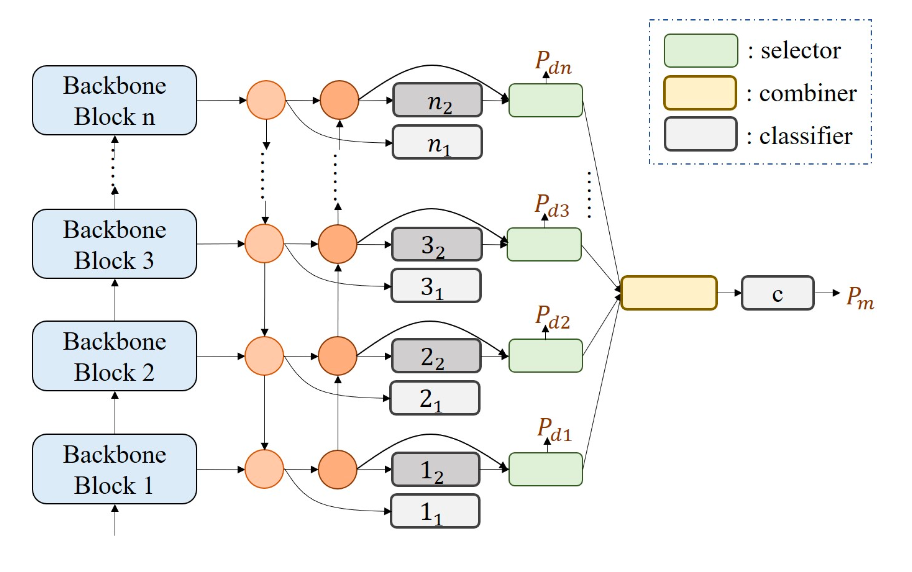
\includegraphics[width=0.95\linewidth]{figure/herbs}
\caption{The architecture of HERBS. Screenshot from \cite{chou2023fine}. ``The circles in the middle part denote the multi-scale feature fusion module, such as Feature Pyramid Network (FPN). The classifiers in the middle are used to generate classification map for background suppression.'' (quote from original paper)}
\label{fig:herbs}
\end{figure}


\subsection{Hyperparameters}
% epoch, temperature, lambda, optimizer, scheduler

\subsubsection{Image size, batch size and epochs}

All images will first be resized to $384 \times 384$ before being sent into models. This can reduce computing resources, which is also a common practice in image classification.

The batch size is set to 16, which can fit in our GPU.

As for epochs, all models used for experiments and evaluation are trained for 80 epochs. I further trained the model to 120 epochs for better performance;	 this model is also the submitted one.

\subsubsection{Feature Pyramid Network and Number of selected features}


Feature Pyramid Network (FPN) is the component for extracting the features generated by backbones. The number of features in each level of FPN is 1536.

And the numbers of selected features for layer 1 to layer 4 are 256, 128, 64 and 32, respectively.


\subsubsection{Weights of Loss}

In HERBS, they design multiple loss terms, each for different components. In this project, I won't modify these weights, because tuning them requires high computational resources. And the effect of tuning the weights is also unknown. Therefore, I will use the same value as original paper.

\begin{itemize}
\item $\lambda_{m}$ = 1
\item $\lambda_{d}$ = 5
\item $\lambda_{l}$ = 0.3
\item $\lambda_{r}$ = 1
\end{itemize}


\subsubsection{Temperature}

In the official code, the temperature in a given epoch is calculated by,

\begin{equation}
\text{Temperature} = \text{Init. Temperature} \cdot (0.5^{\lfloor\frac{\text{epoch}}{10}\rfloor}).
\end{equation}

The above equation is actually equivalent with the equation in the paper.

\autoref{fig:temp} further demonstrate the temperature over epoch. 

\begin{figure}[H]
\centering
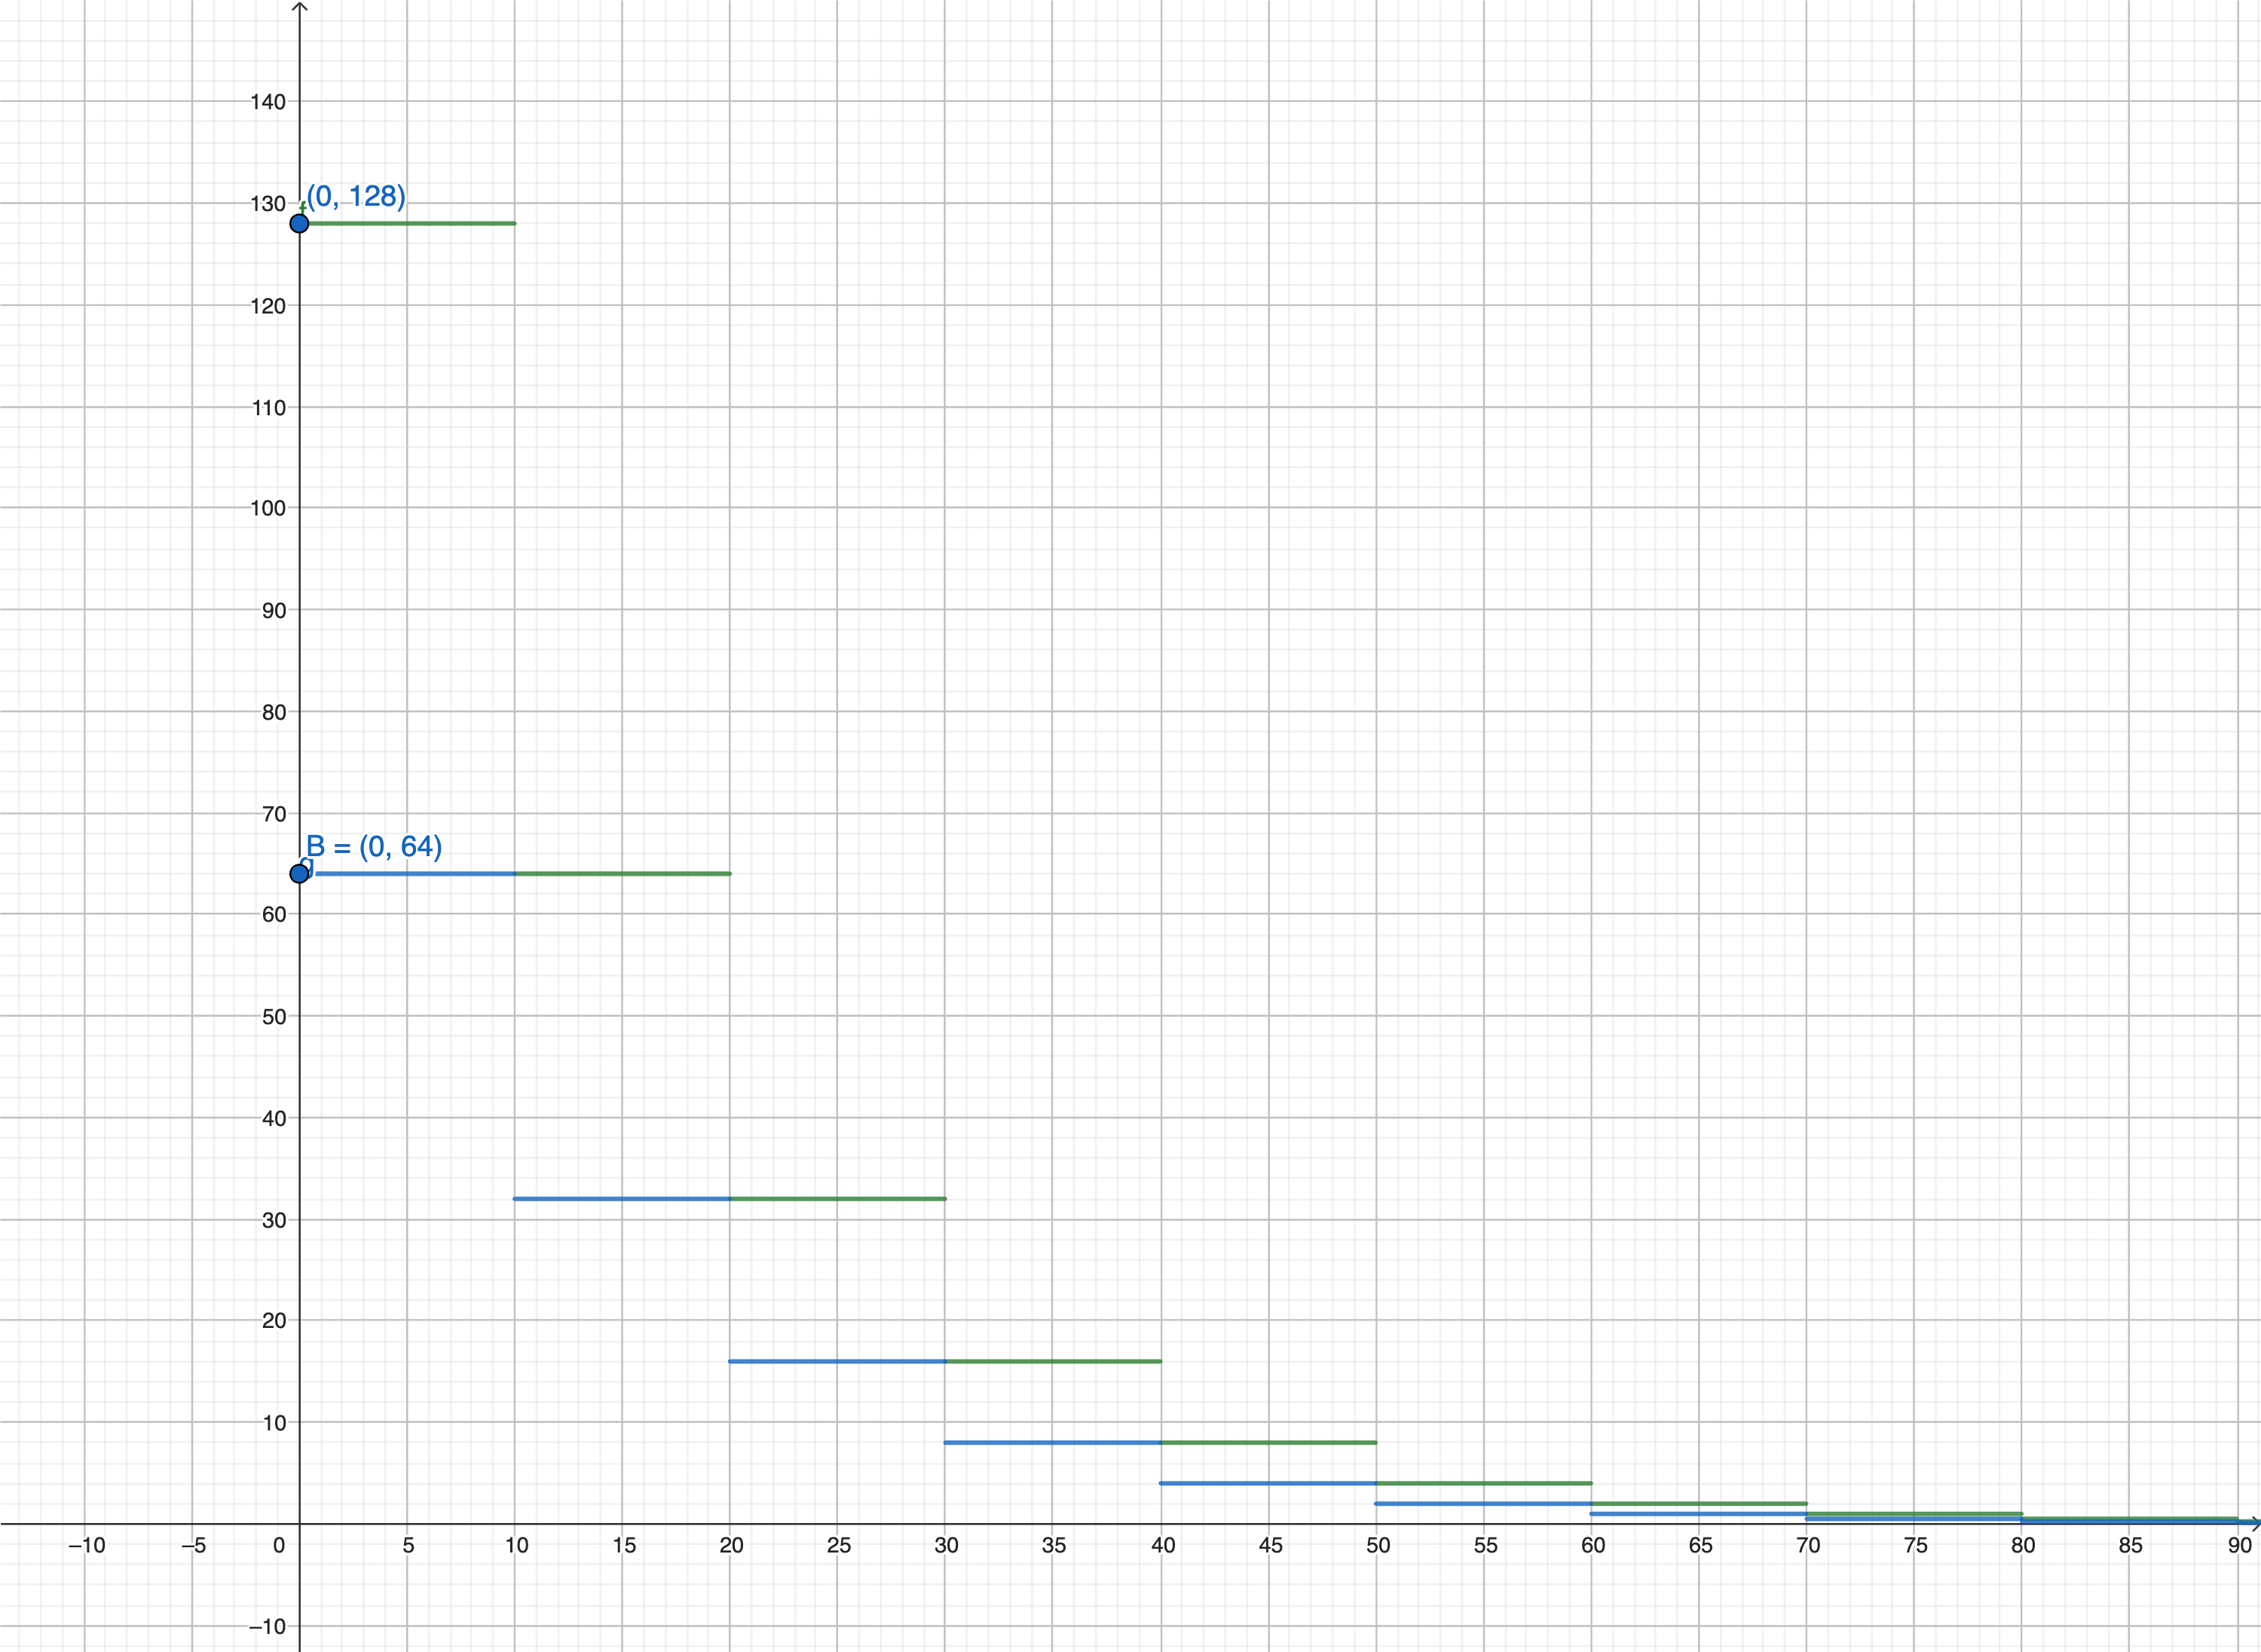
\includegraphics[width=0.95\linewidth]{figure/temp_plot}
\caption{The temperature from 0 to 80 epochs, the blue line is temperature=64, the green line is temperature=128}
\label{fig:temp}
\end{figure}

\subsection{Training Strategy}
% lr plot, temperature, warm up



\subsubsection{Optimizer}

The official code used SGD as the optimizer. In \autoref{sec: exp}, I will conduct a experiment and discuss the difference of using SGD and AdamW.

The parameters of SGD are:

\begin{itemize}
\item \texttt{momentum = 0.9}
\item \texttt{max\_lr = 0.0005}
\item \texttt{weight\_decay = 0.0003}
\item \texttt{nesterov = True}
\end{itemize}

\subsubsection{Learning Rate and Warm-up Batches}

As we can see in \autoref{fig:lr}, the learning rate is initially set low, this is because of the introducing of warm-up batches. This concept first be introduced in \cite{goyal2017accurate}. This idea is that the weights of the model are initialized randomly, thus, the gradient of model's weights may be unstable. Therefore, if we first make the learning rate lower in the early stage of training, the model can see all the data without updating the weight too much. After the model sees all the data, we can fallback to normal learning rate scheduling. In this way, we can reduce the probability of falling into local minima.

The learning rate scheduler used in HERBS's official code is cosine decay. 

The number of warm-up batches is 1500.

\begin{figure}[H]
\centering
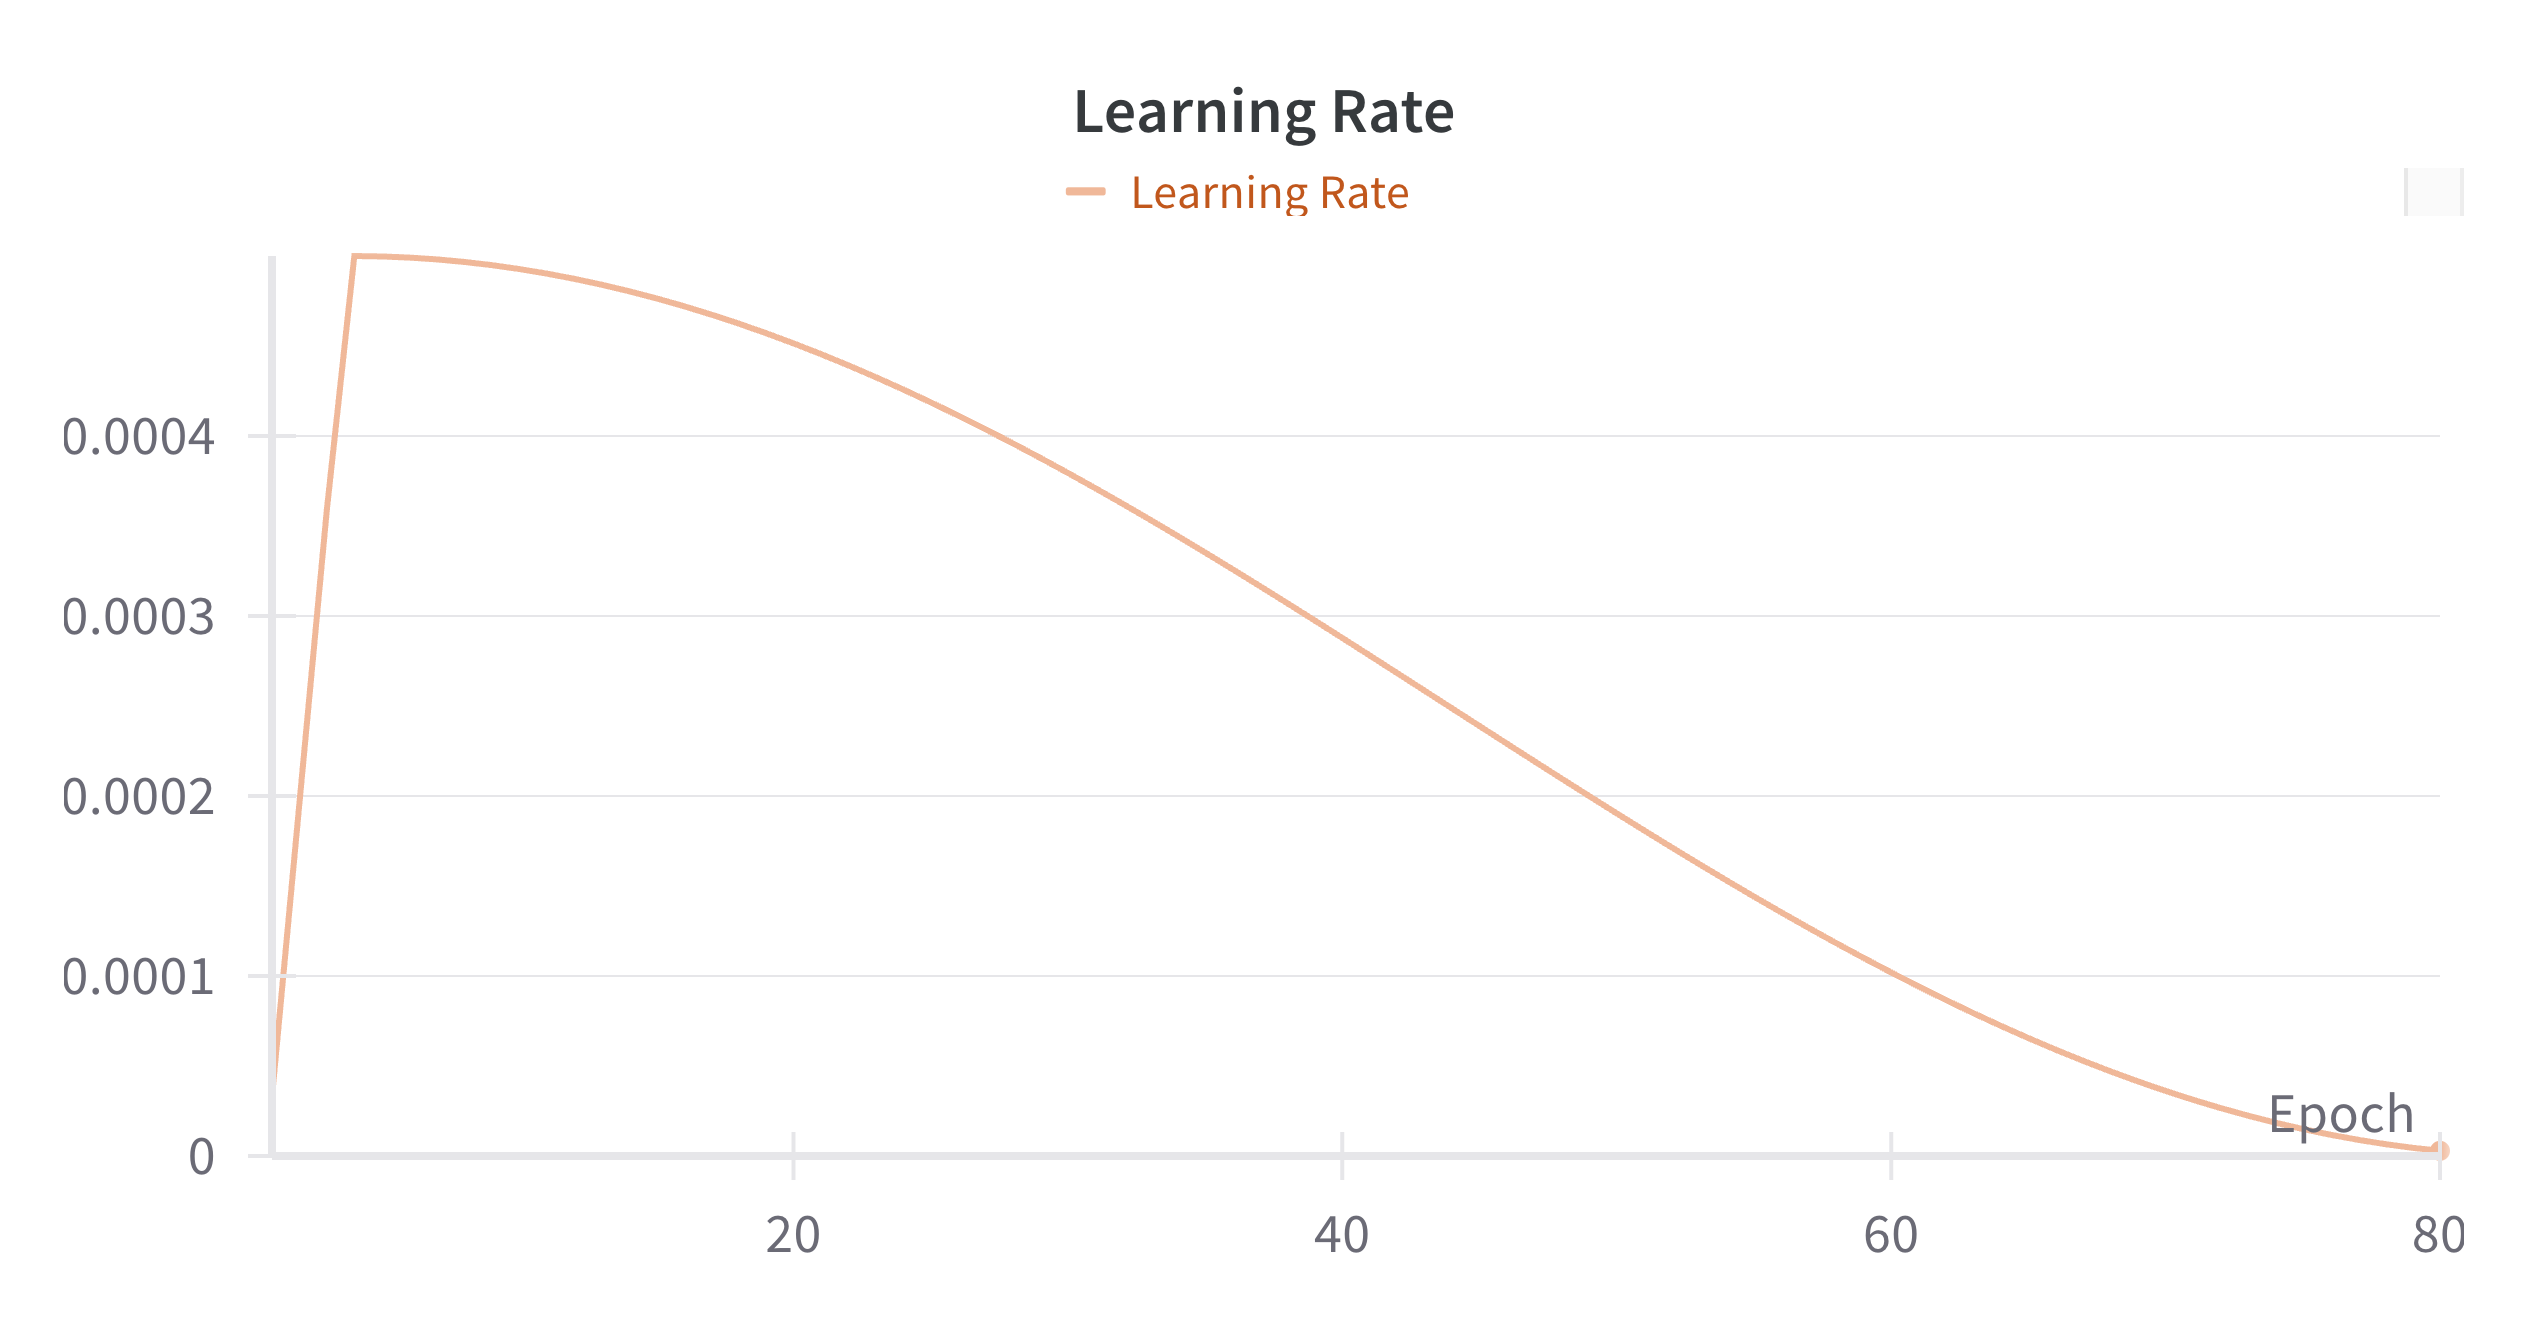
\includegraphics[width=0.95\linewidth]{figure/lr}
\caption{The learning rate overtime from 0 to 80 epoches.}
\label{fig:lr}
\end{figure}


\subsubsection{Data Argumentation}

The training time augmentation is aligned with HERBS's official code, as shown in \autoref{code: dataaug}.
\begin{code}
\captionof{listing}{Training Time Data Argumentation}
\label{code: dataaug}
\begin{minted}
transforms.Resize((510, 510), Image.BILINEAR),
transforms.RandomCrop((384, 384)),
transforms.RandomHorizontalFlip(),
transforms.RandomApply([transforms.GaussianBlur(kernel_size=(5, 5), sigma=(0.1, 5))], p=0.1),
transforms.RandomAdjustSharpness(sharpness_factor=1.5, p=0.1),
transforms.ToTensor(),
transforms.Normalize(mean=[0.485, 0.456, 0.406], std=[0.229, 0.224, 0.225])
\end{minted}
\end{code}

In my opinion, I believe that this data argumentation is strong enough, I've tried adding other data argumentation, like color jitter, but didn't achieve better performance. In addition, I think applying data argumentation that would change the color in the image would make the model unable to correctly classify images. This is because color is a critical part when we classify different birds.

It's noteworthy that the mean and standard deviation used in normalization are calculated based on ImageNet\cite{deng2009imagenet}, which is a common practice in image classification. Adding the normalization term can stable the training process.



\section{Experiments\label{sec: exp}}

\subsection{Evaluation Method}

Because the provided datasets only contains a labeled training set and a unlabeled test set, it's hard to evaluate the model's performance. Thus, I randomly split the original training set to a training set and validation set using 8/2 split. For the experiments provides below, I trained the model using the smaller training set, and use the validation set for evaluation. This is possible because every image in validation set is labeled.

For evaluation metric, I mainly use accuracy and F1-score to evaluate the performance of models.

Moreover, following the evaluation in HERBS\cite{chou2023fine}, I also performed evaluation on fined-class. In particular, I will use 9 generic classes, including flycatcher, gull, kingfisher, sparrow, tern, vireo, warbler, woodpecker, wren. The mapping between each generic classes and species will be listed in \autoref{sec: bonus}.


\subsection{Ablation Study}

In this section, I will mainly discuss about one component and one hyperparameter in HERBS, which are combiner and temperature.

By adjusting these two configurations, I trained 4 models, which are, 

\begin{enumerate}
\item With combiner, temperature=64 (default setting)
\item With combiner, temperature=128
\item Without combiner, temperature=64
\item Without combiner, temperature=128
\end{enumerate}

\begin{table}[H]
\centering
\caption{Ablation study on combiner and temperature. The F1-score is calculated with a weighted manner.}
\label{tab:ablation}
\begin{tabular}{|cc|c|l|}
\hline
\multicolumn{2}{|c|}{Model}                    & \multirow{2}{*}{Accuracy} & \multirow{2}{*}{F1-score} \\ \cline{1-2}
\multicolumn{1}{|c|}{Combiner}   & Temperature &                           &                           \\ \hline
\multicolumn{1}{|c|}{\checkmark} & 64          & 0.9235                    & 0.9227                    \\ \hline
\multicolumn{1}{|c|}{\checkmark} & 128         & \textbf{0.9245}                    & \textbf{0.9238}                    \\ \hline
\multicolumn{1}{|c|}{}           & 64          & 0.9216                    & 0.908                     \\ \hline
\multicolumn{1}{|c|}{}           & 128         & 0.9144                    & 0.912                     \\ \hline
\end{tabular}
\end{table}


\begin{figure}[H]
\centering
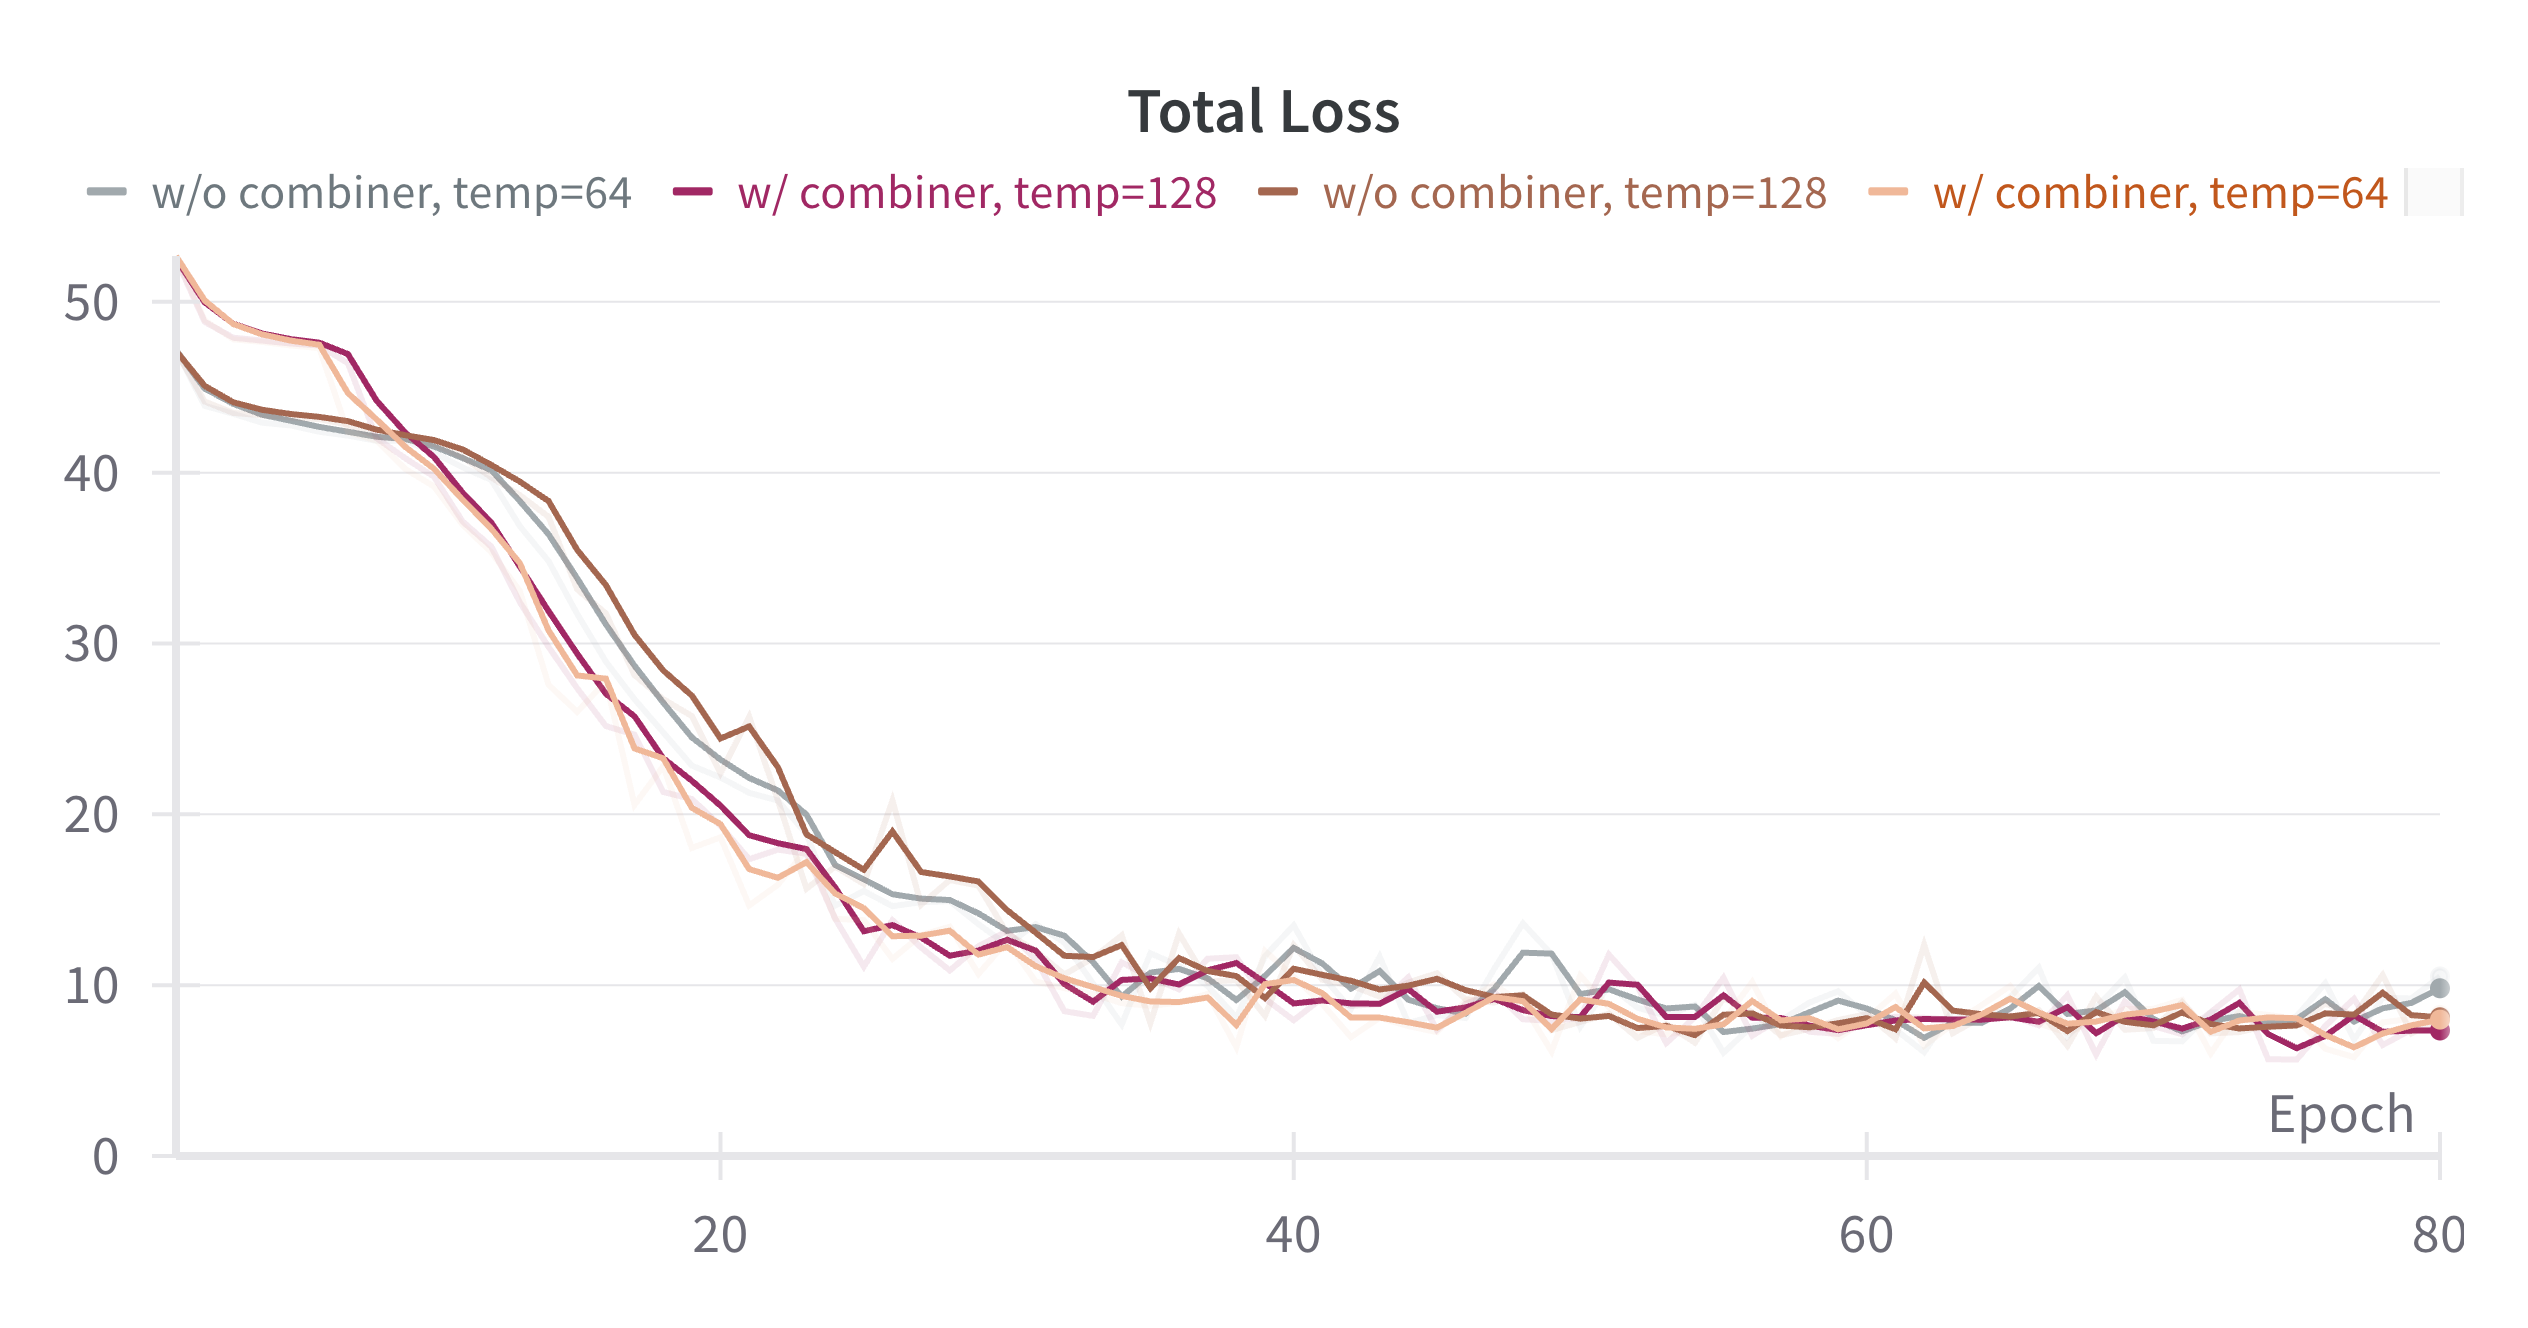
\includegraphics[width=0.95\linewidth]{figure/loss}
\caption{The training loss of four models over time}
\label{fig:ablloss}
\end{figure}


As we can see in \autoref{tab:ablation}, the performance of the model with combiner, temperature=128 is the best, achieving the accuracy of $0.9245$. This might due to the high exploration rate in features in the early phase of training. However, I believe that tuning the temperature is not very useful, the increasing randomness of selecting features may not directly improve the performance. As for the combiner, it's clear that the accuracy decrease after removing the combiner, for both low and high temperature. Therefore, this ablation study proves that the combiner introduced in HERBS has positive effect in performance.

For training loss, we can observe in \autoref{fig:ablloss}, the loss of four models are all decreasing and finally converge to nearly the same value. We can also notice that the loss of two high temperature model are higher in first 10 epochs, but quickly decreased afterward. I think this is mainly because of the diversity of features in the early stage of training.

Finally, I will use model with combiner and temperature=128 to conduct following experiments, because it has the highest accuracy and F1-score.

\subsection{Inference Time Transformation}

It's a common practice to perform some transformations on image when inference. In evaluation, I will perform several type of transformation combinations, to evaluate how transformations effect final result.

I tested three inference time transformation on the model with default setting. \textbf{Original transformation} is the implementation used in HERBS's official code, which first resize the image to $510 \times 510$ and center crop the image to $384 \times 384$; This transformation is also a common practice in image classification. \textbf{No crop transformation} directly resize the image to $384 \times 384$. \textbf{Five crop transformation} first resize the image to $510 \times 510$, and then crop the image into four corners and the central crop.

\begin{code}
\captionof{listing}{Original Transformation}
\begin{minted}
transforms.Resize((510, 510), Image.BILINEAR),
transforms.CenterCrop((384, 384)),
transforms.ToTensor(),
transforms.Normalize(mean=[0.485, 0.456, 0.406], std=[0.229, 0.224, 0.225])
\end{minted}
\end{code}

\begin{code}
\captionof{listing}{No Crop Transformation}
\begin{minted}
transforms.Resize((384, 384), Image.BILINEAR),
transforms.Lambda(lambda crops: transforms.ToTensor(),
transforms.Normalize(mean=[0.485, 0.456, 0.406], std=[0.229, 0.224, 0.225])
\end{minted}
\end{code}

\begin{code}
\captionof{listing}{Five Crop Transformation}
\begin{minted}
transforms.Resize((510, 510), Image.BILINEAR),
transforms.FiveCrop((384, 384)),
transforms.Lambda(lambda crops: torch.stack([transforms.ToTensor()(crop) for crop in crops])),
transforms.Lambda(lambda crops: torch.stack([transforms.Normalize(mean=[0.485, 0.456, 0.406],std=[0.229, 0.224, 0.225])(crop) for crop in crops]))
\end{minted}
\end{code}

I tested the above three kinds of transformations on the model with default hyperparameters. \autoref{tab:trans} shows the results, five crop can improve the accuracy by 0.001, compared with original transformation.

\begin{table}[H]
\centering
\caption{The accuracy and F1-score using different transformation methods. The F1-score is calculated in weighed manner.}
\label{tab:trans}
\begin{tabular}{|c|c|c|}
\hline
\textbf{Transformation} & \textbf{Accuracy} & \textbf{F1-score} \\ \hline
Original                & 0.9245            & \textbf{0.9238}   \\ \hline
No Crop                 & 0.9189            & 0.9176            \\ \hline
Five Crop               & \textbf{0.9255}   & \textbf{0.9238}   \\ \hline
\end{tabular}
\end{table}


\subsection{Generic Classes}

In this section, I will mainly discuss about the accuracy within generic class. This experiment is useful because we can observe species in which generic class are more similar, thus the model can't distinguish than very well.

As we can observe in \autoref{tab:generic}, the accuracy within ``Gull'' class is significant lower than other classes. In \autoref{fig:species}, each kinds of gull is looks very similar, I think this is why the accuracy is the lowest in this class.

I further plot the confusion matrices for each generic class in \autoref{sec:confusion}.


\begin{table}[H]
\centering
\caption{The precision and number of false positive samples for each generic class.}
\label{tab:generic}
\begin{tabular}{|c|c|c|}
\hline
\textbf{Generic Class} & \textbf{Precision} & \textbf{FP} \\ \hline
Flycatcher    & 0.81429   & 8  \\ \hline
Gull          & 0.79487   & 1  \\ \hline
Kingfisher    & 0.9       & 0  \\ \hline
Sparrow       & 0.89423   & 2  \\ \hline
Tern          & 0.8       & 1  \\ \hline
Vireo         & 0.89855   & 5  \\ \hline
Warbler       & 0.932     & 6  \\ \hline
Woodpecker    & 0.96552   & 0  \\ \hline
Wren          & 0.97143   & 0  \\ \hline
\end{tabular}
\end{table}

\begin{figure}[H]
\centering
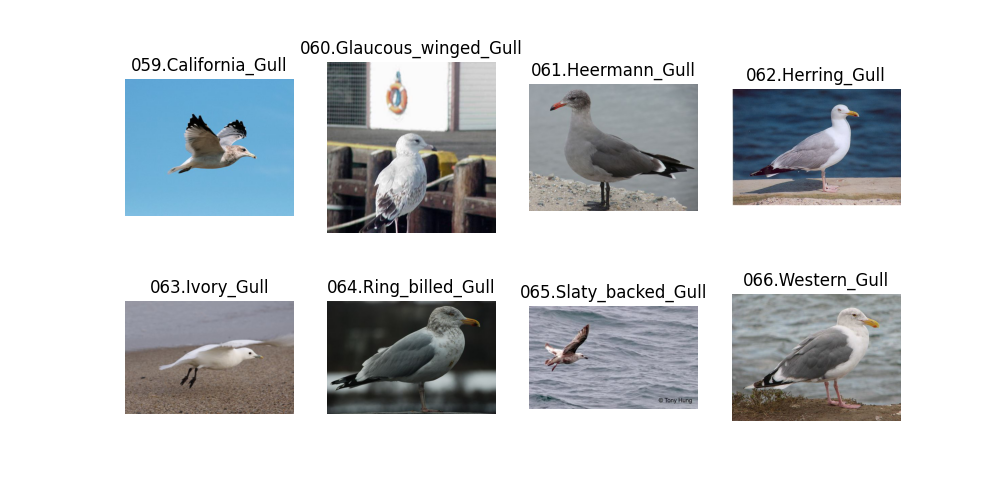
\includegraphics[width=\linewidth]{figure/species}
\caption{Each kind of gulls in the datasets.}
\label{fig:species}
\end{figure}




\section{Bonus\label{sec: bonus}}

\subsection{Training the model}

You should able to train the model by running, \\
\texttt{python main.py --c ./configs/config.yaml}.

I've also provided the configuration files I used for every experiment.

\subsection{Running the the inference code}

I used Jupyter Notebook for inference, because I can test it on Google Colab before submitting. If TAs want to run the notebook on Google Colab, the process is as follow:

\begin{enumerate}
\item Open \texttt{110550088\_inference.ipynb} in Google Colab
\item Upload all files and directories in the zip file to Colab, placed them in \texttt{/content}.
\item Download model's weights from Google Drive link, and upload it to \texttt{/content}.
\item Now, the \texttt{/content} should look like \autoref{fig:colabfile}.
\item I put the test datasets in \texttt{training/datasets/test}. Therefore, it's no need to download the test datasets.
\item Finally, after running all cells in the notebook, you should able to see \texttt{submission.csv} appears in the folder.
\end{enumerate}

Also, after testing, I found that there is no need to install additional packages when running in colab. Though I still provide the \texttt{requirements.txt}, I don't use pip to install them in the jupyter notebook.

Noted that the use T4 GPU runtime in Google Colab, my inference notebook needs to run under environment with GPU.

\begin{figure}[H]
\centering
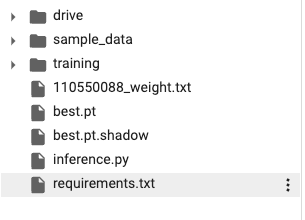
\includegraphics[width=0.95\linewidth]{figure/colabfile}
\caption{The screenshot after completing step 3.}
\label{fig:colabfile}
\end{figure}


\subsection{Future Work}

I think that the performance of HERBS is actually bounded by the size of training data. The accuracy in my own experiments is always lower than the number in \cite{chou2023fine}. Also, as mentioned in class, transformer-based model requires more data for training in order to achieve strong performance. Thus, for future work, I would like to figure out if there has any way to improve the data argumentation, let the model can learn even from small amount of data.


\subsection{Confusion Matrix of Each Generic Class\label{sec:confusion}}

In this section, I will provide the confusion matrices within each generic class. By them, we can observe what kinds of species are more likely to be wrongly classified. As I mentioned previously, gulls are very hard to distinguish, this can be also proved in \autoref{fig:evalhightempgull}.


\begin{figure}[H]
\centering
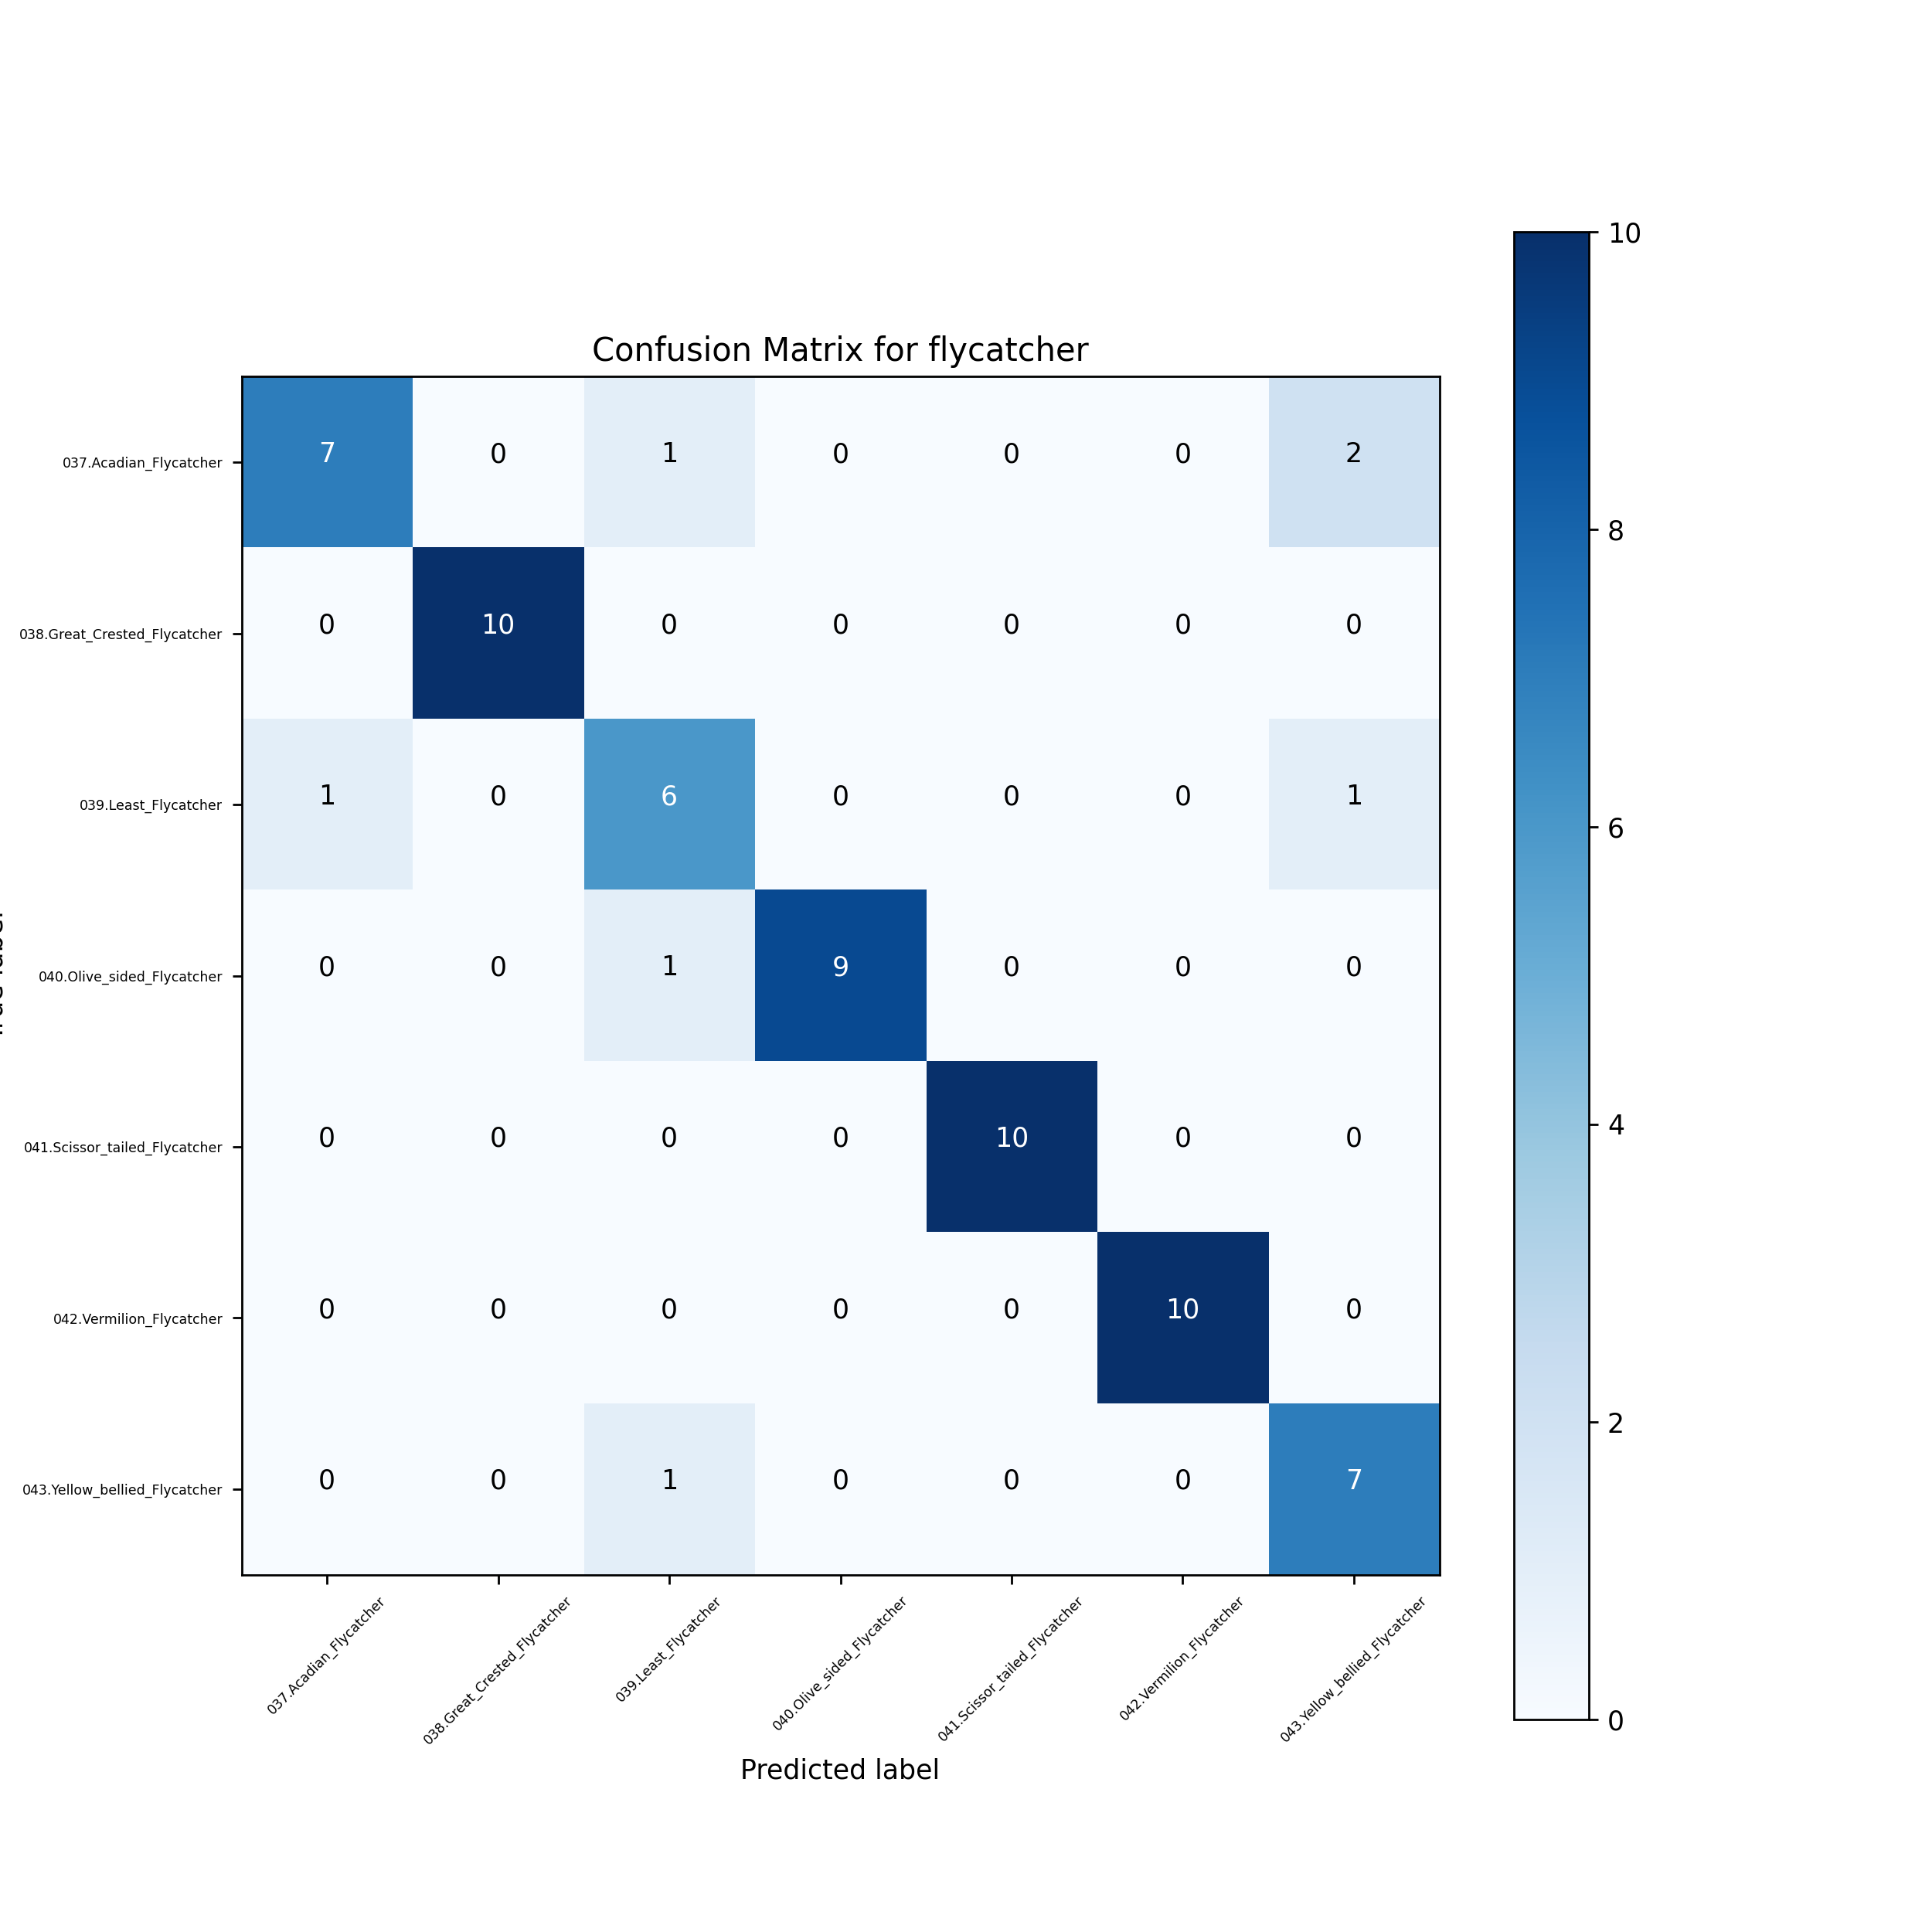
\includegraphics[width=0.95\linewidth]{figure/eval_high_temp_flycatcher}
\caption{The confusion matrix of flycatchers}
\label{fig:evalhightempflycatcher}
\end{figure}
\begin{figure}[H]
\centering
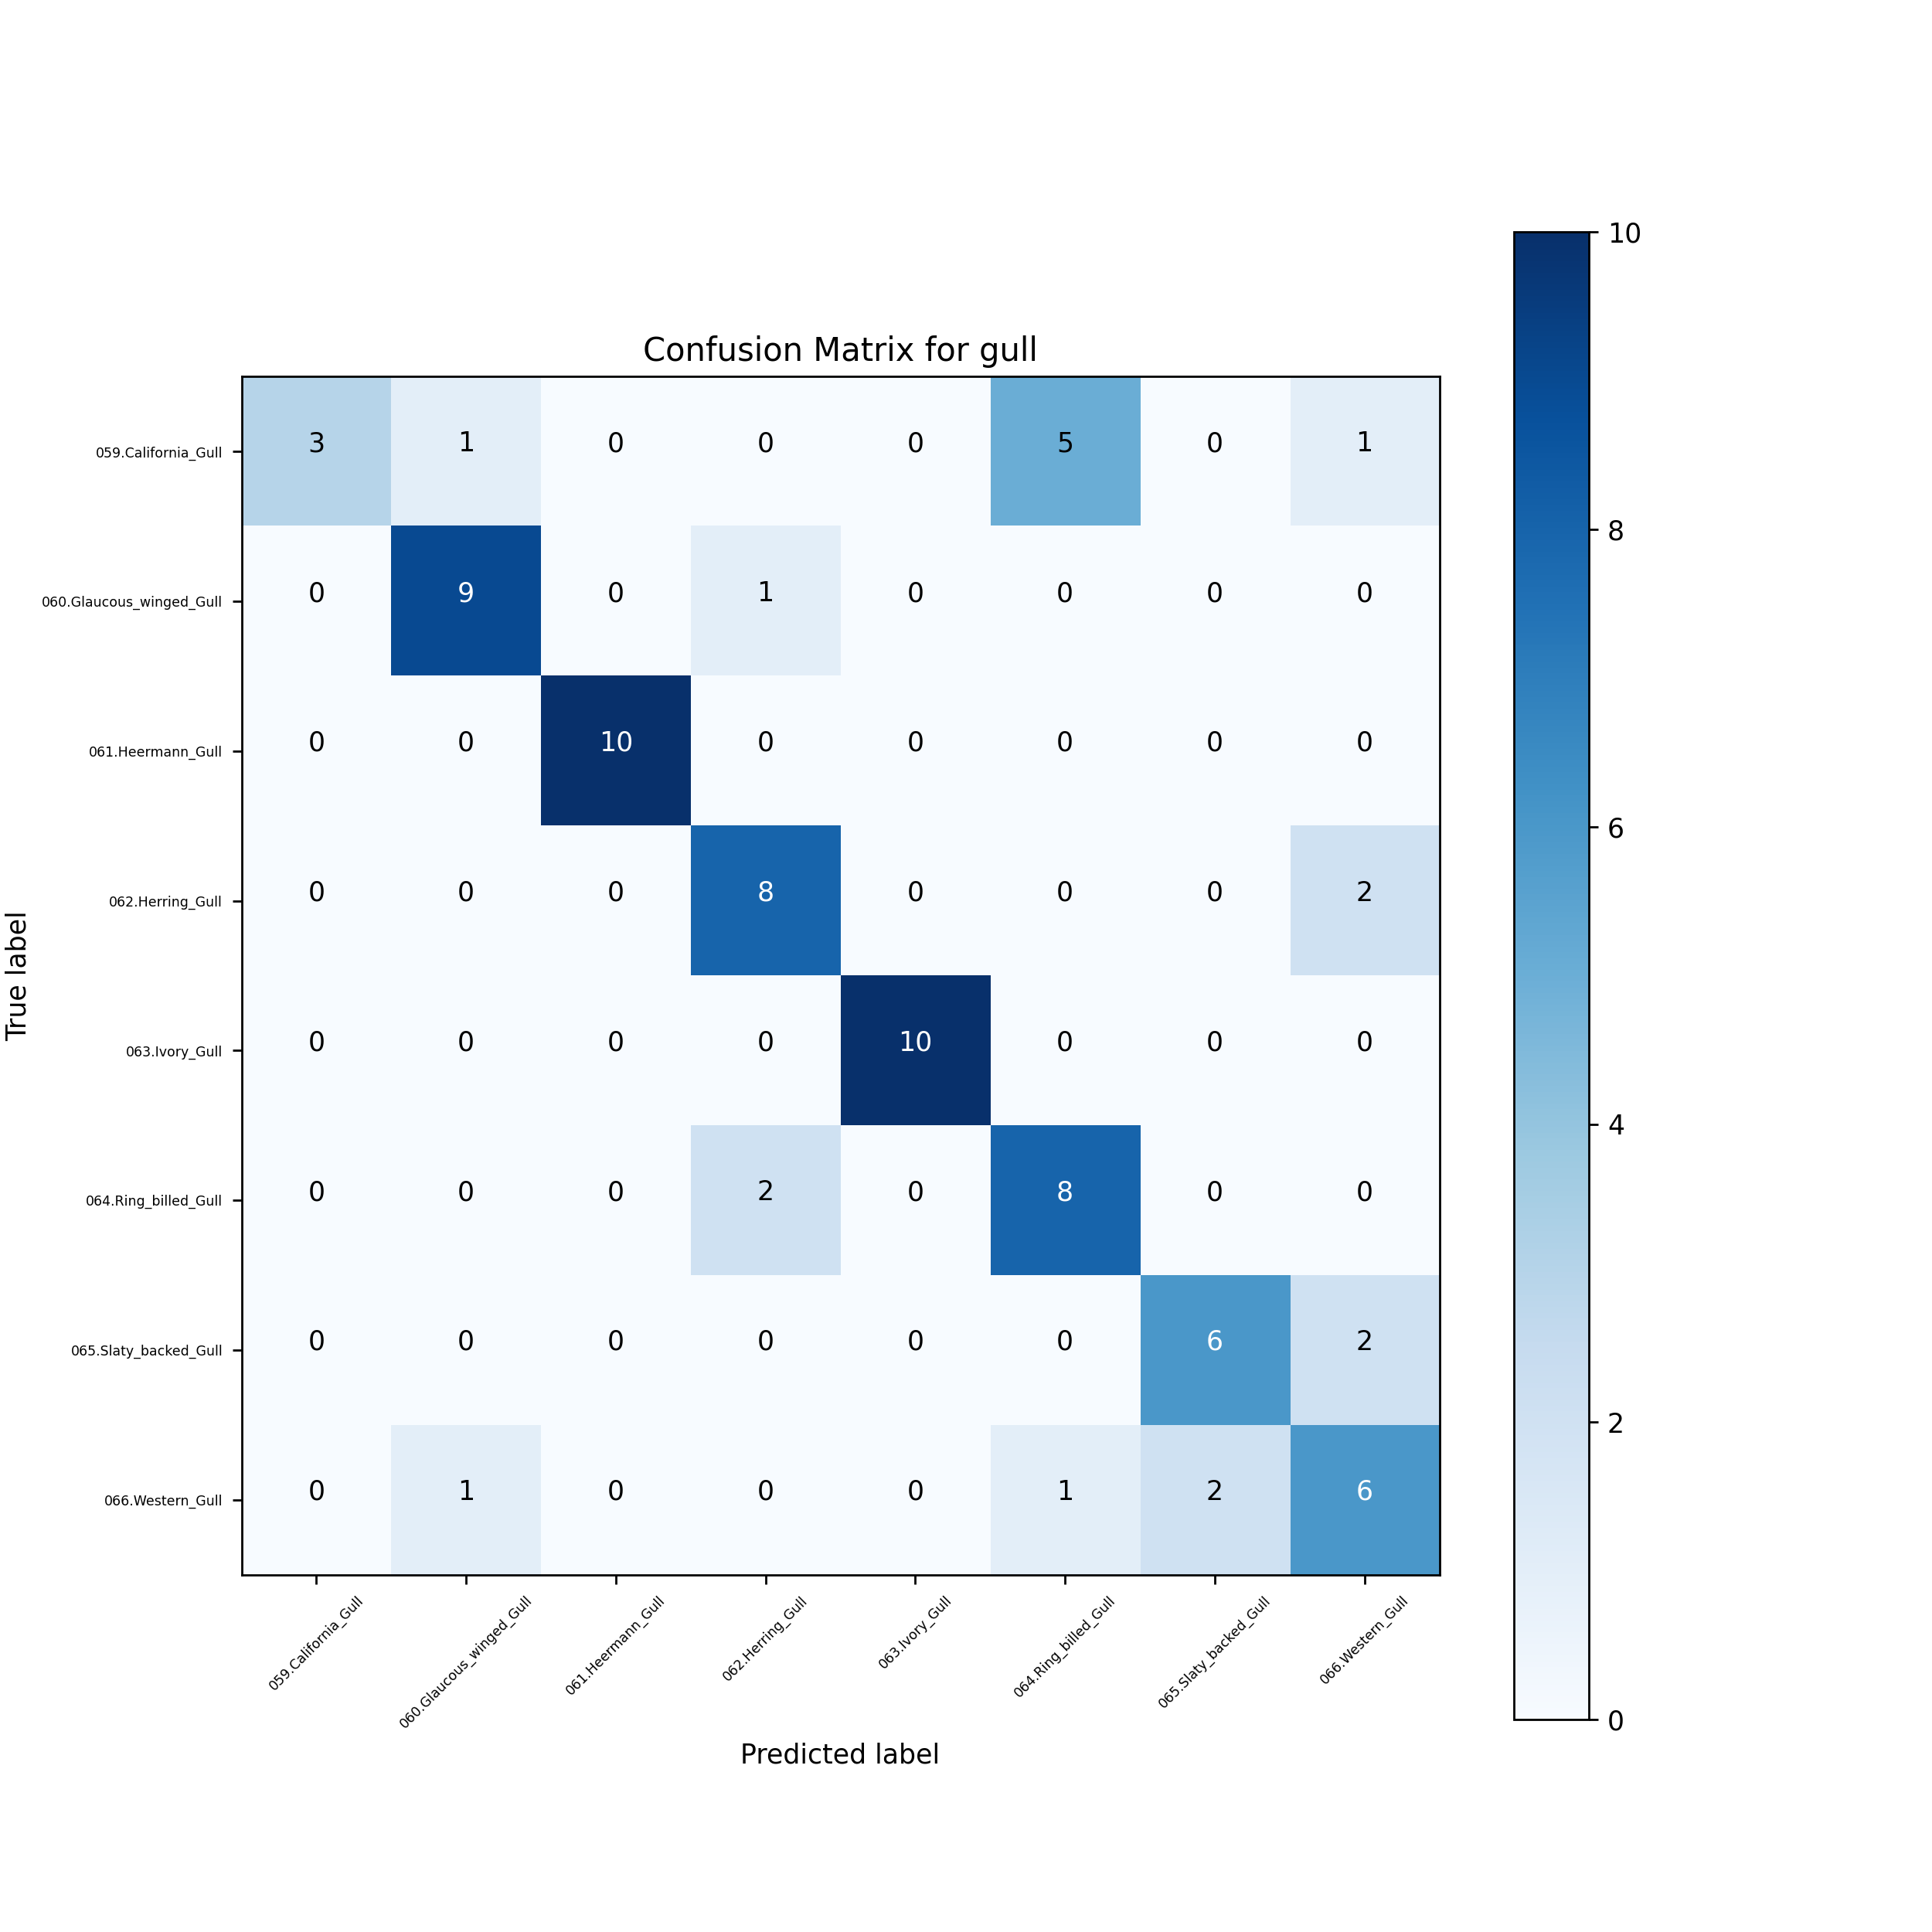
\includegraphics[width=0.95\linewidth]{figure/eval_high_temp_gull}
\caption{The confusion matrix of gulls}
\label{fig:evalhightempgull}
\end{figure}
\begin{figure}[H]
\centering
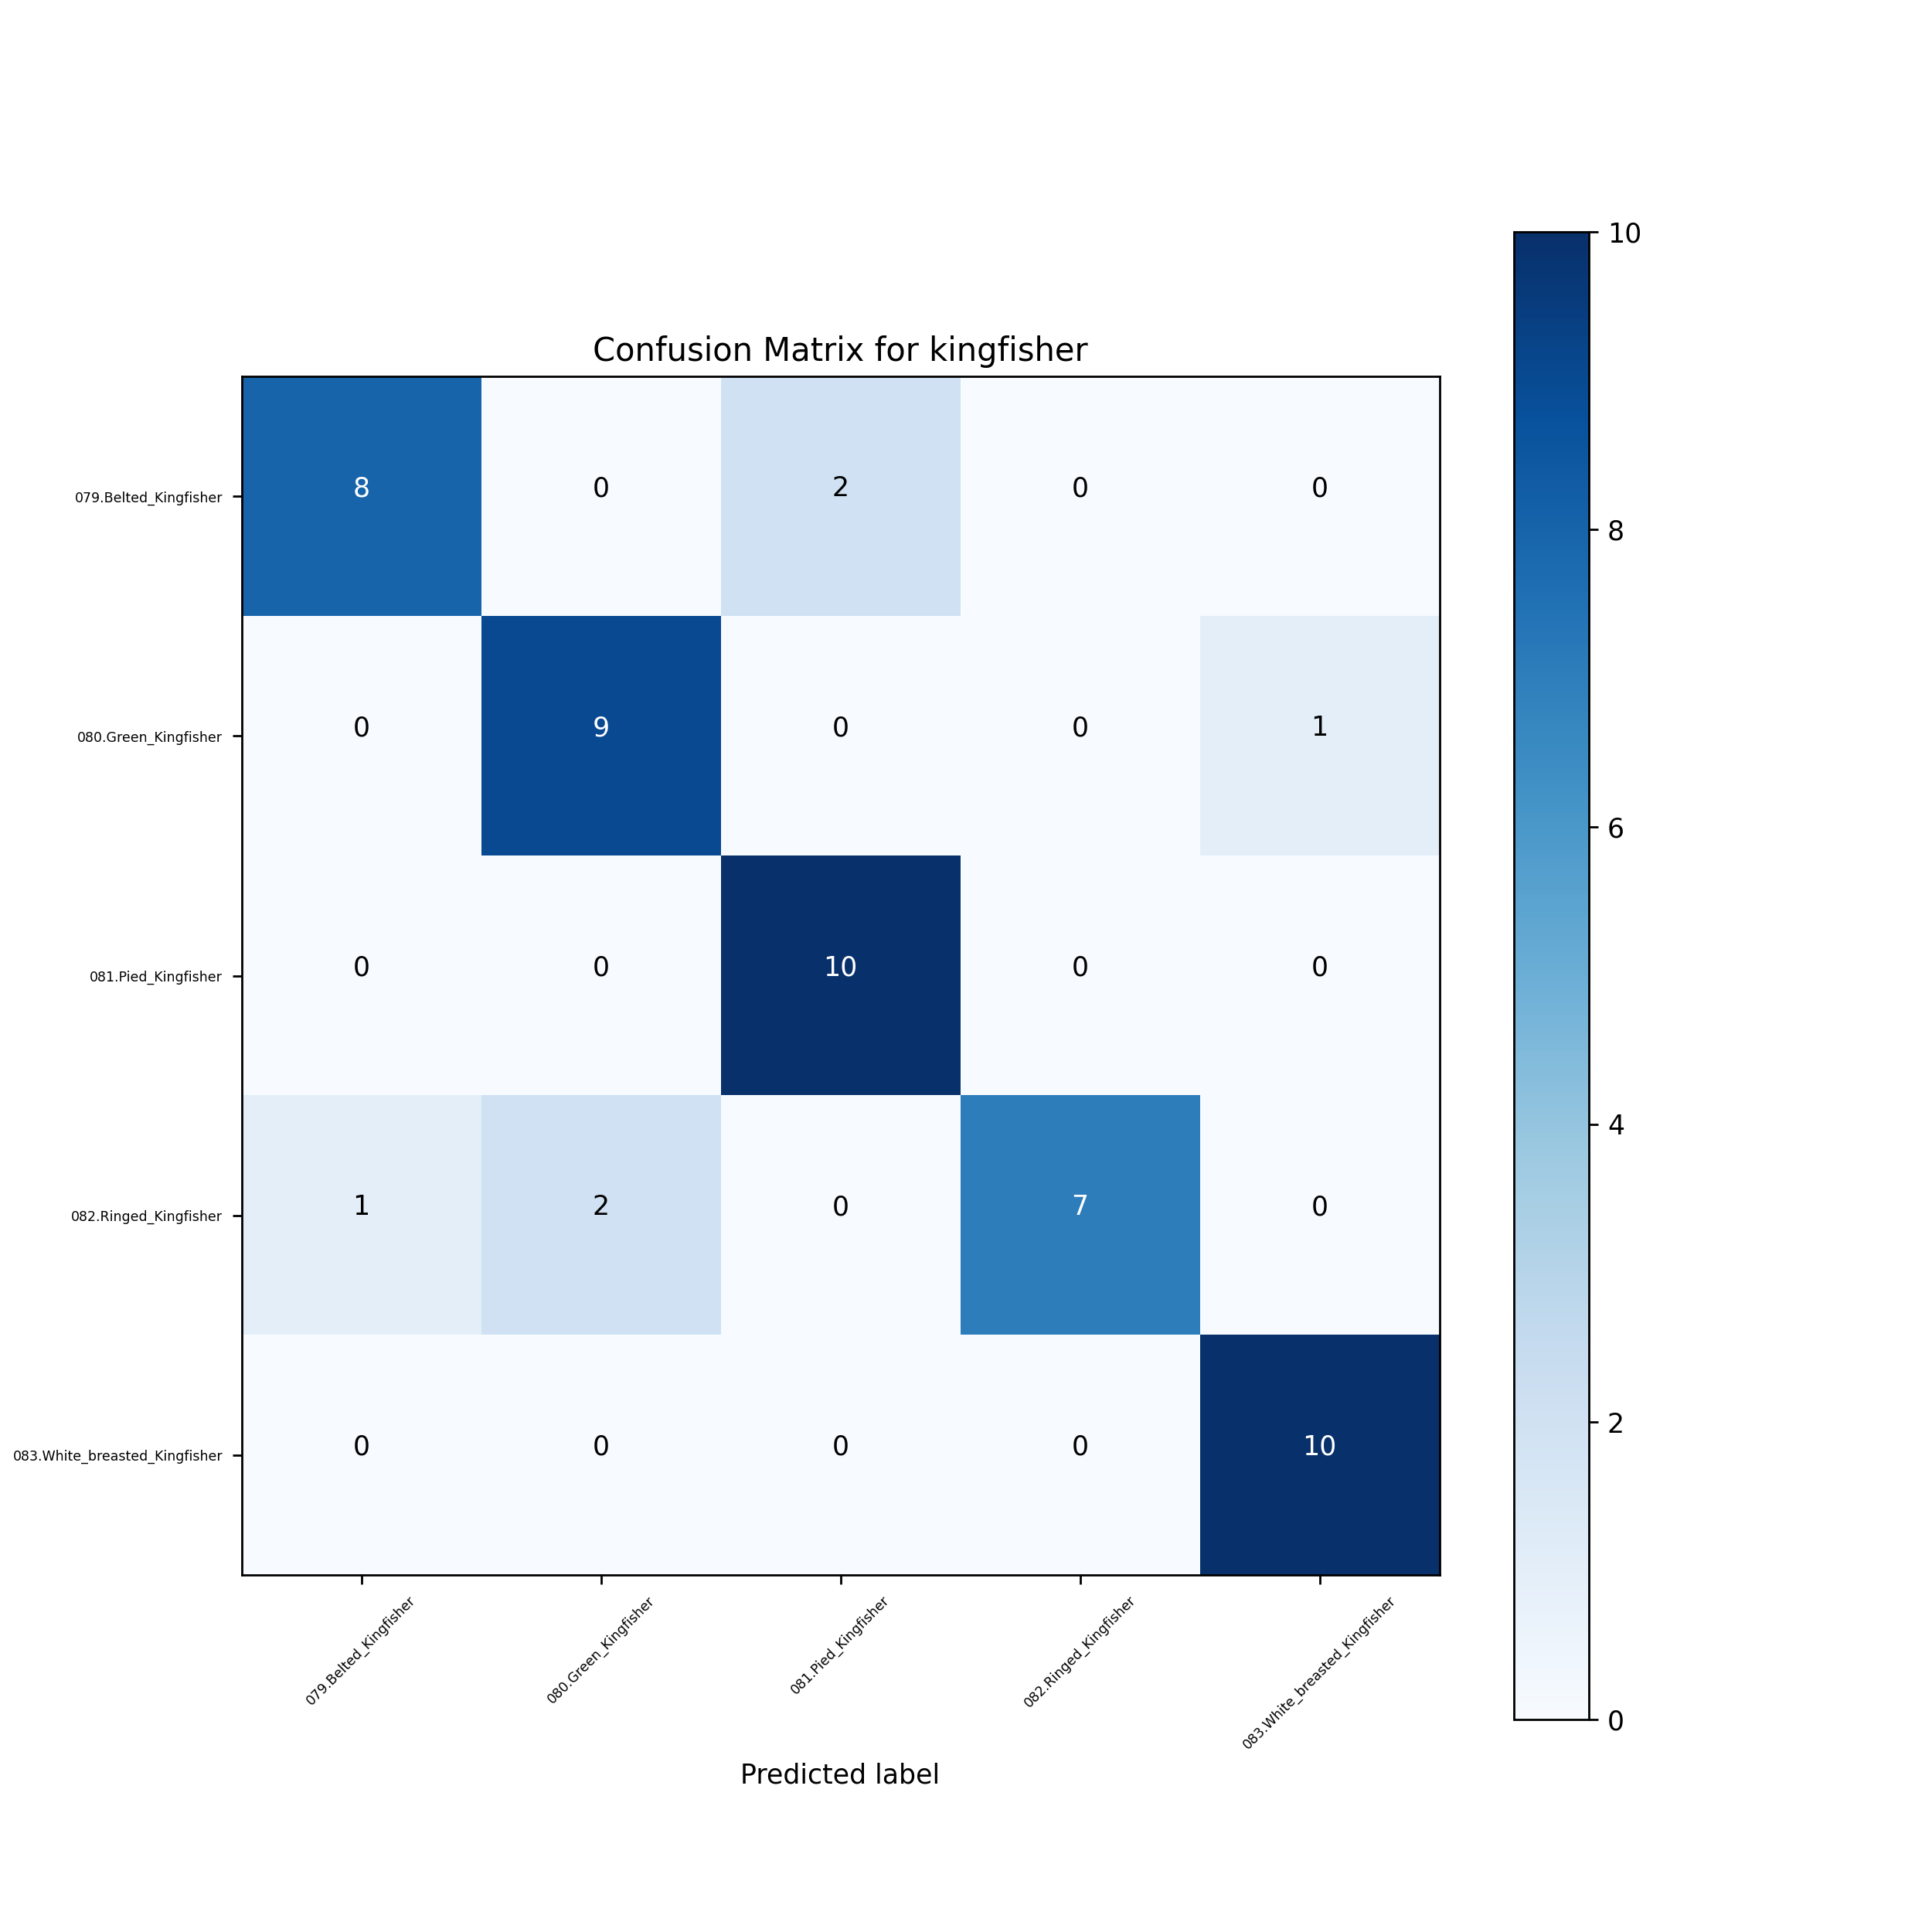
\includegraphics[width=0.95\linewidth]{figure/eval_high_temp_kingfisher}
\caption{The confusion matrix of kingfishers}
\label{fig:evalhightempkingfisher}
\end{figure}
\begin{figure}[H]
\centering
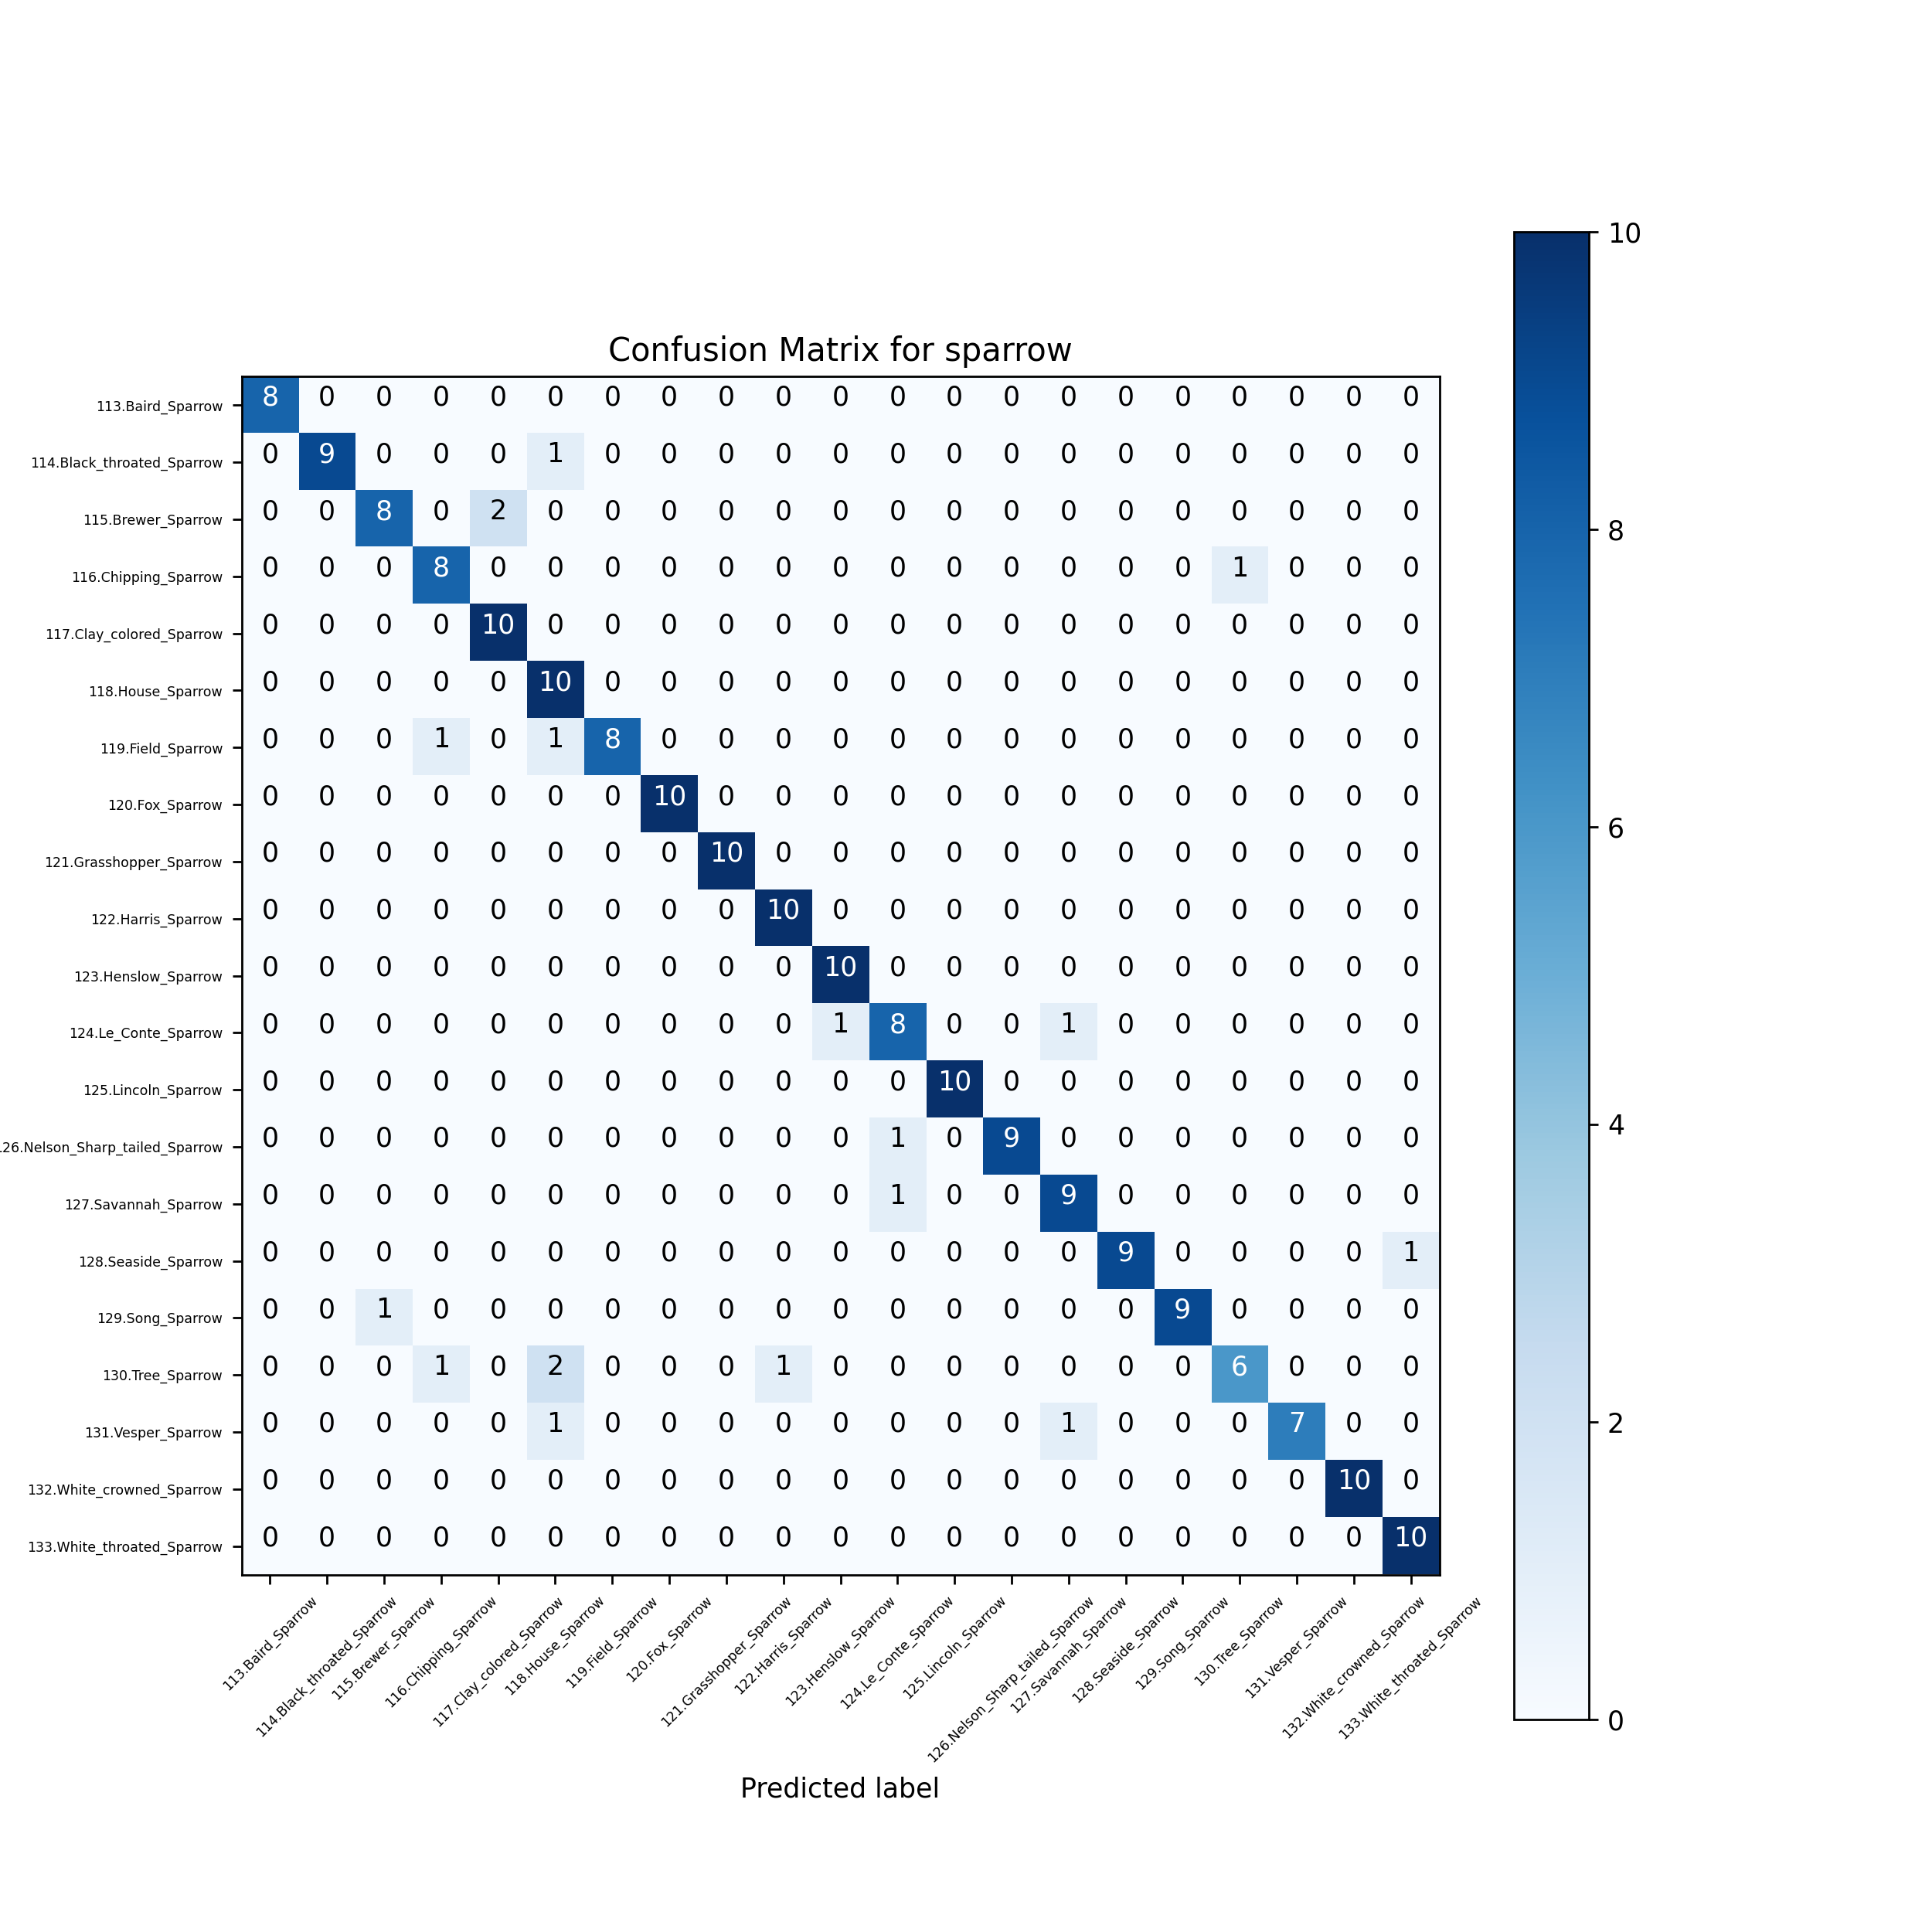
\includegraphics[width=0.95\linewidth]{figure/eval_high_temp_sparrow}
\caption{The confusion matrix of sparrows}
\label{fig:evalhightempsparrow}
\end{figure}
\begin{figure}[H]
\centering
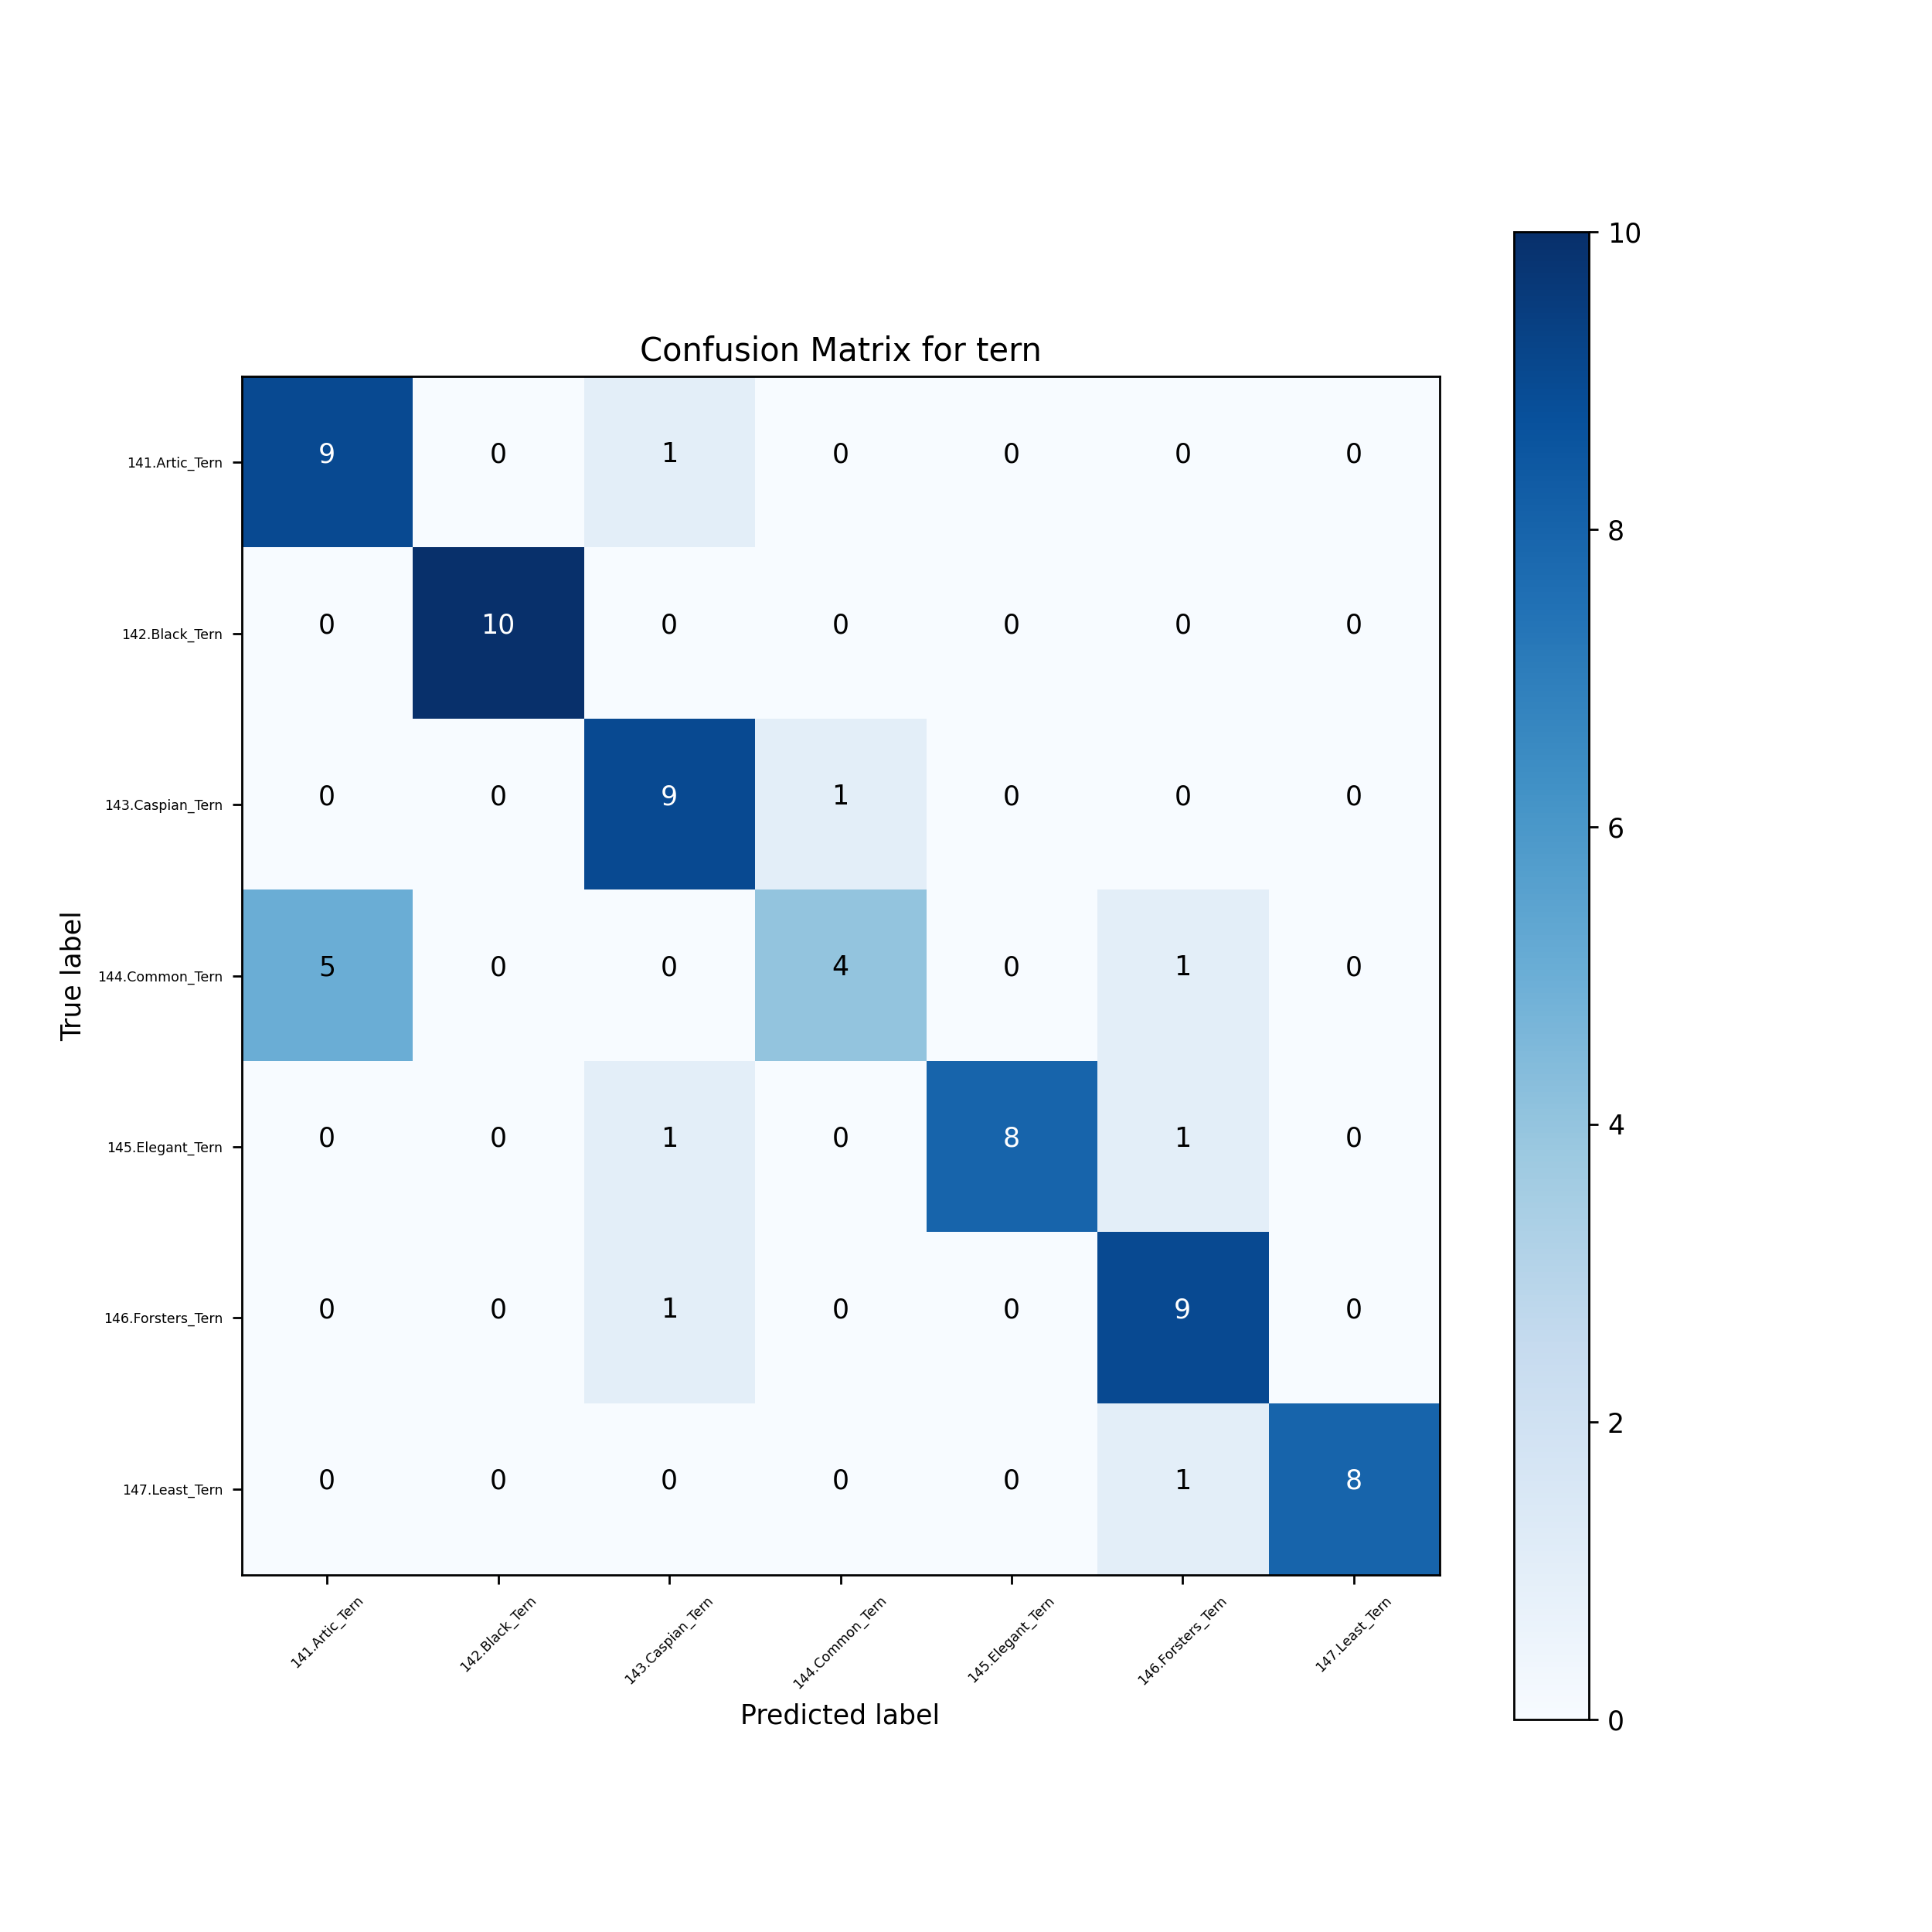
\includegraphics[width=0.95\linewidth]{figure/eval_high_temp_tern}
\caption{The confusion matrix of terns}
\label{fig:evalhightemptern}
\end{figure}
\begin{figure}[H]
\centering
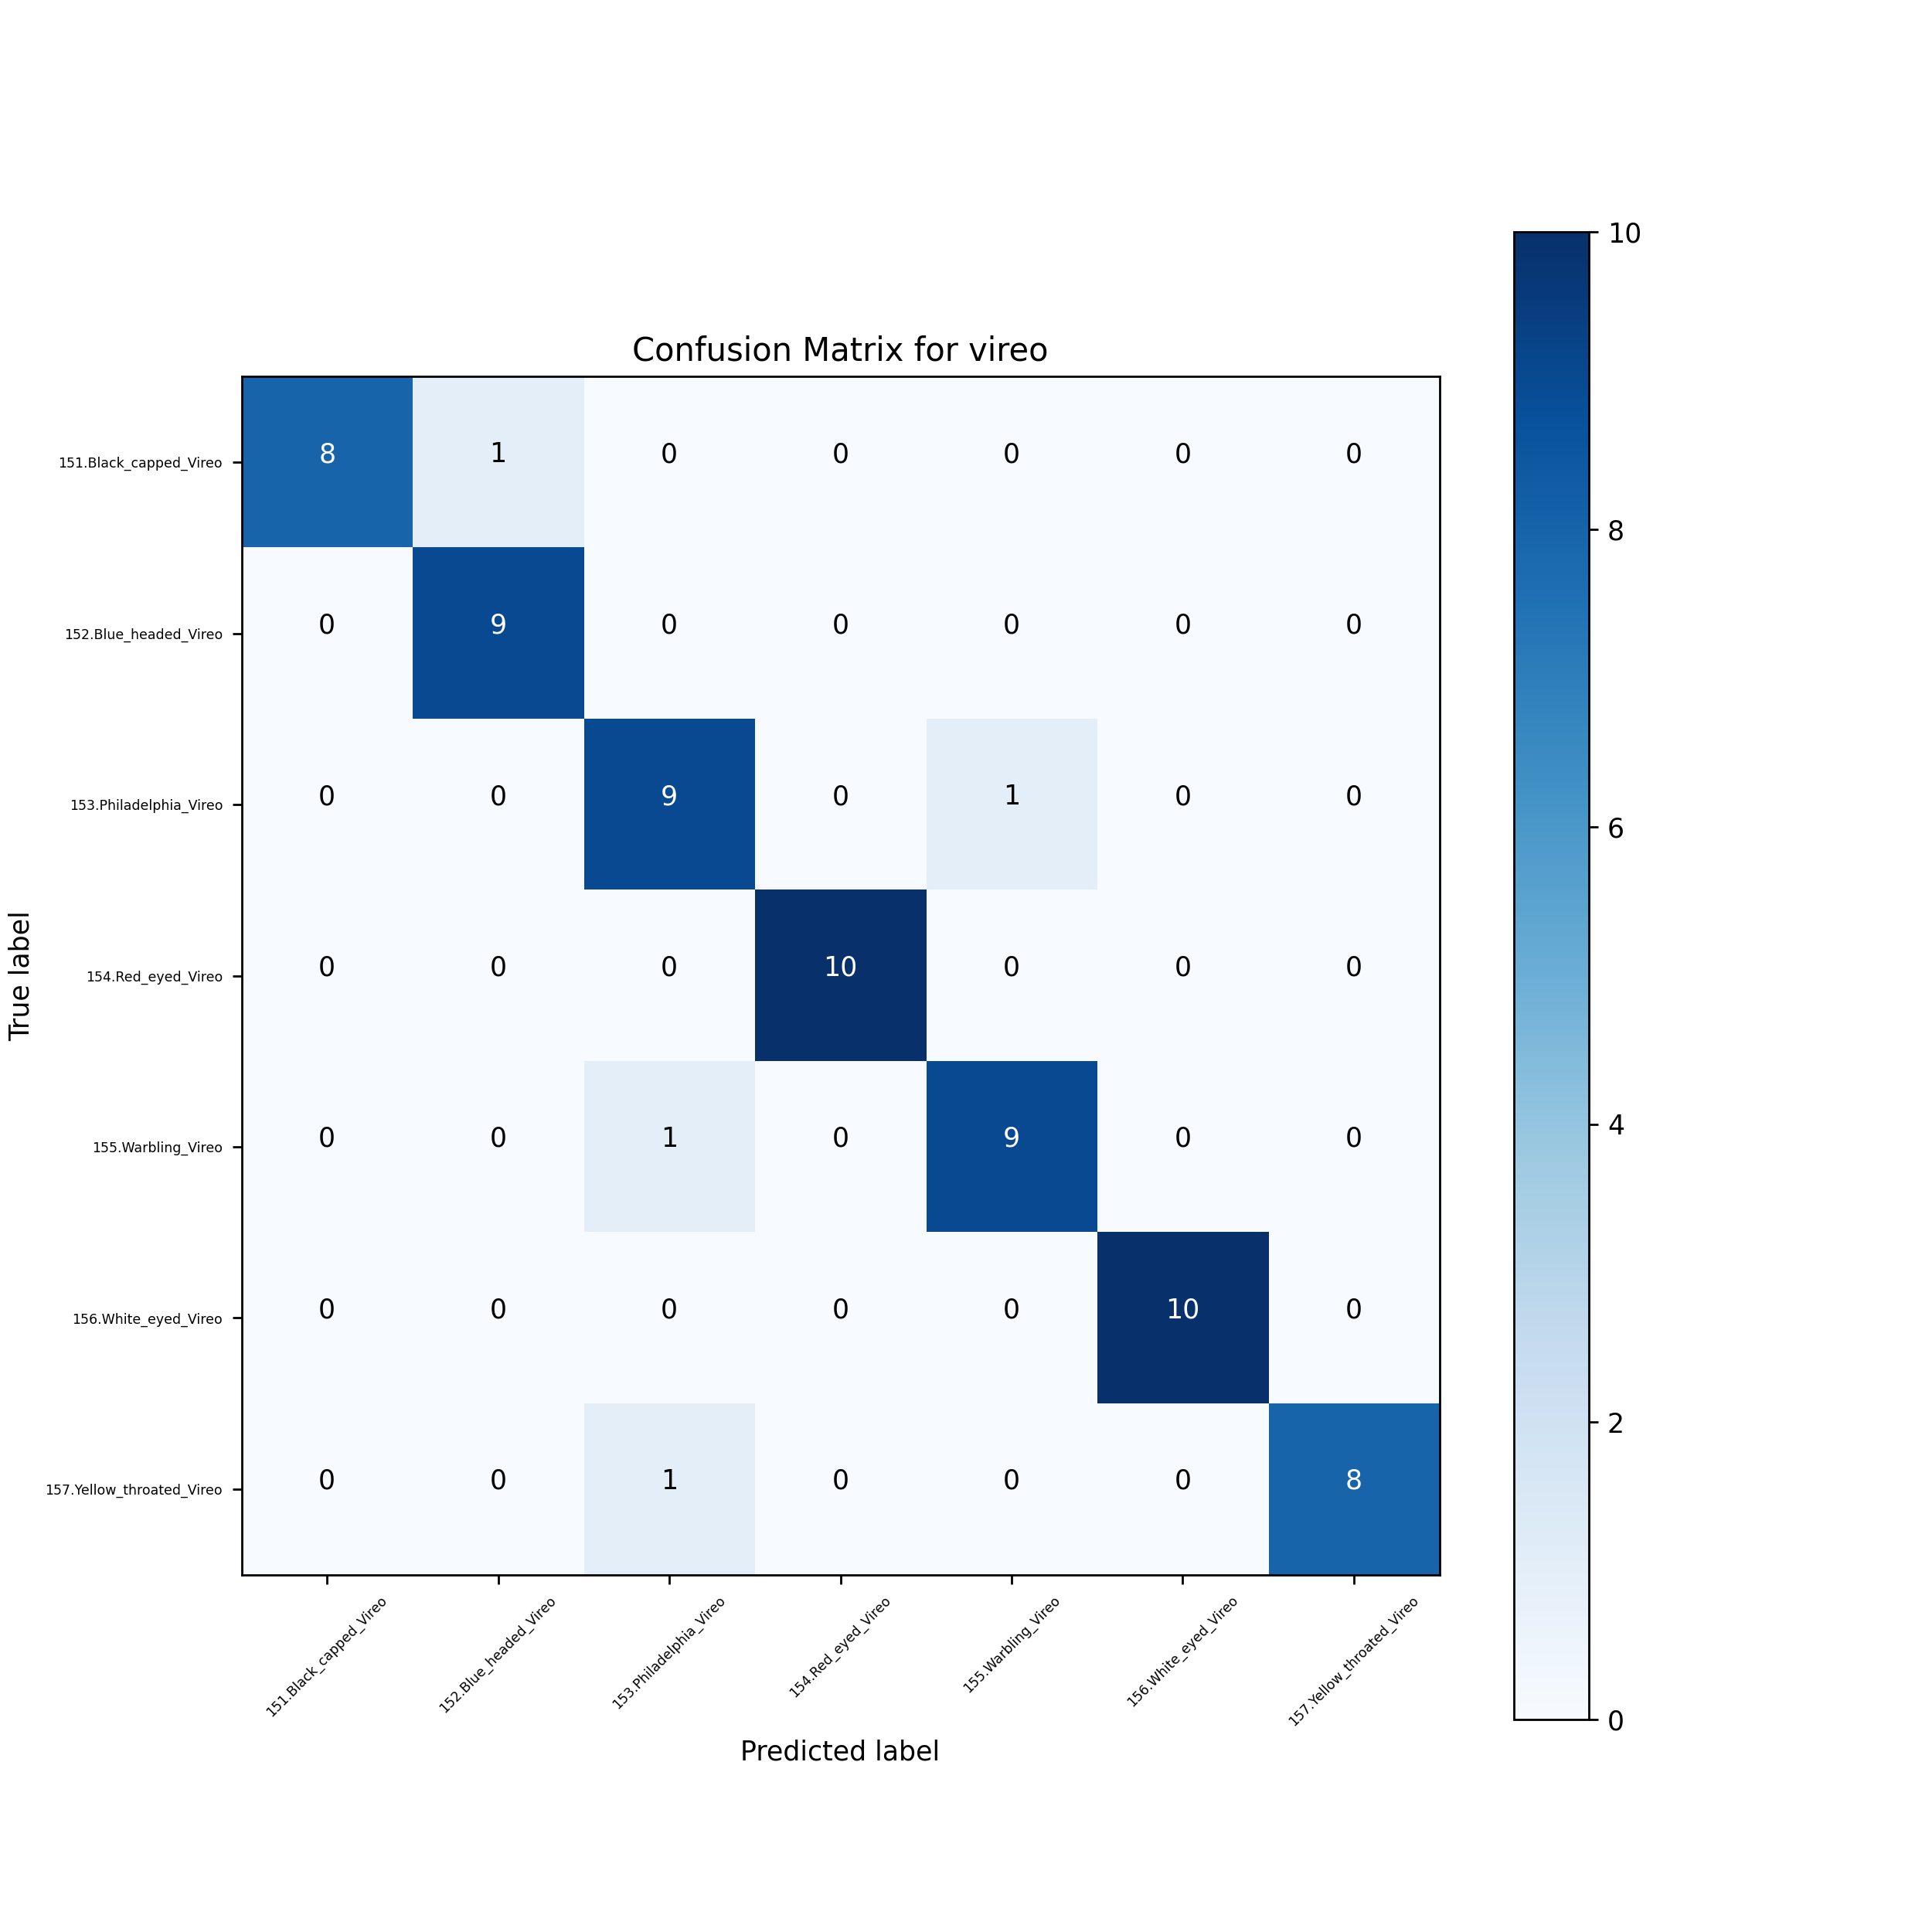
\includegraphics[width=0.95\linewidth]{figure/eval_high_temp_vireo}
\caption{The confusion matrix of vireos}
\label{fig:evalhightempvireo}
\end{figure}
\begin{figure}[H]
\centering
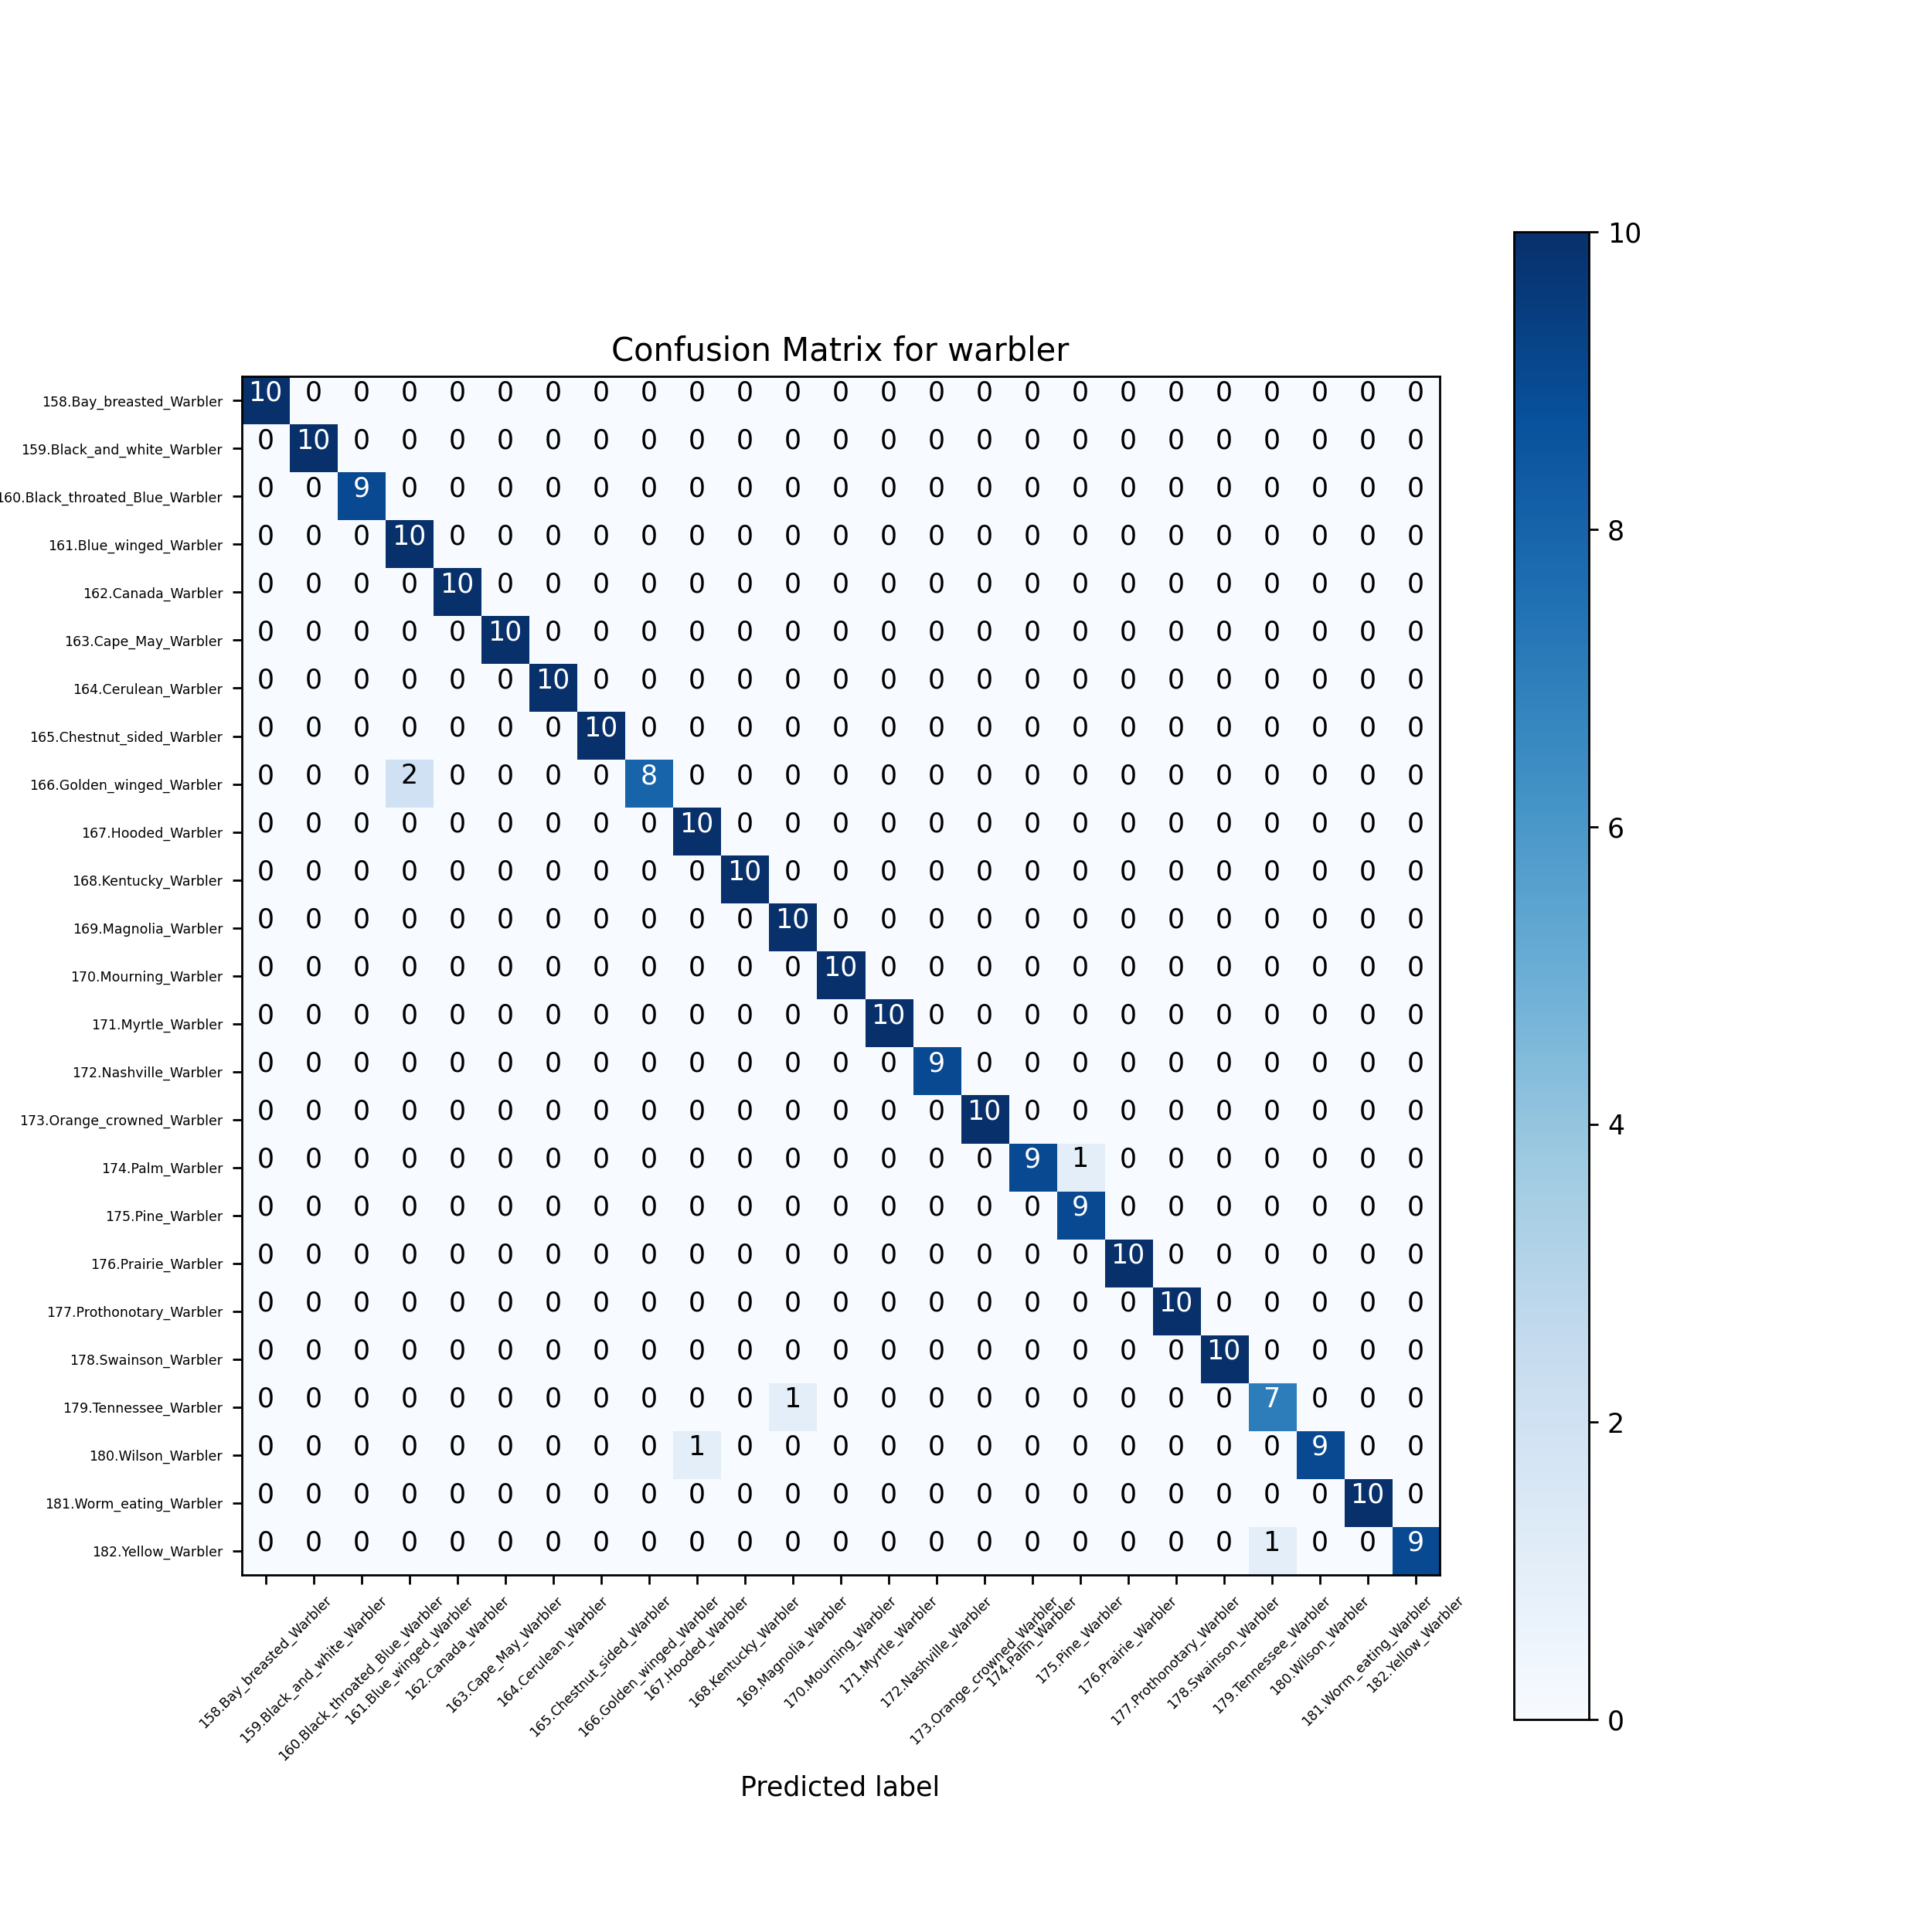
\includegraphics[width=0.95\linewidth]{figure/eval_high_temp_warbler}
\caption{The confusion matrix of warblers}
\label{fig:evalhightempwarbler}
\end{figure}
\begin{figure}[H]
\centering
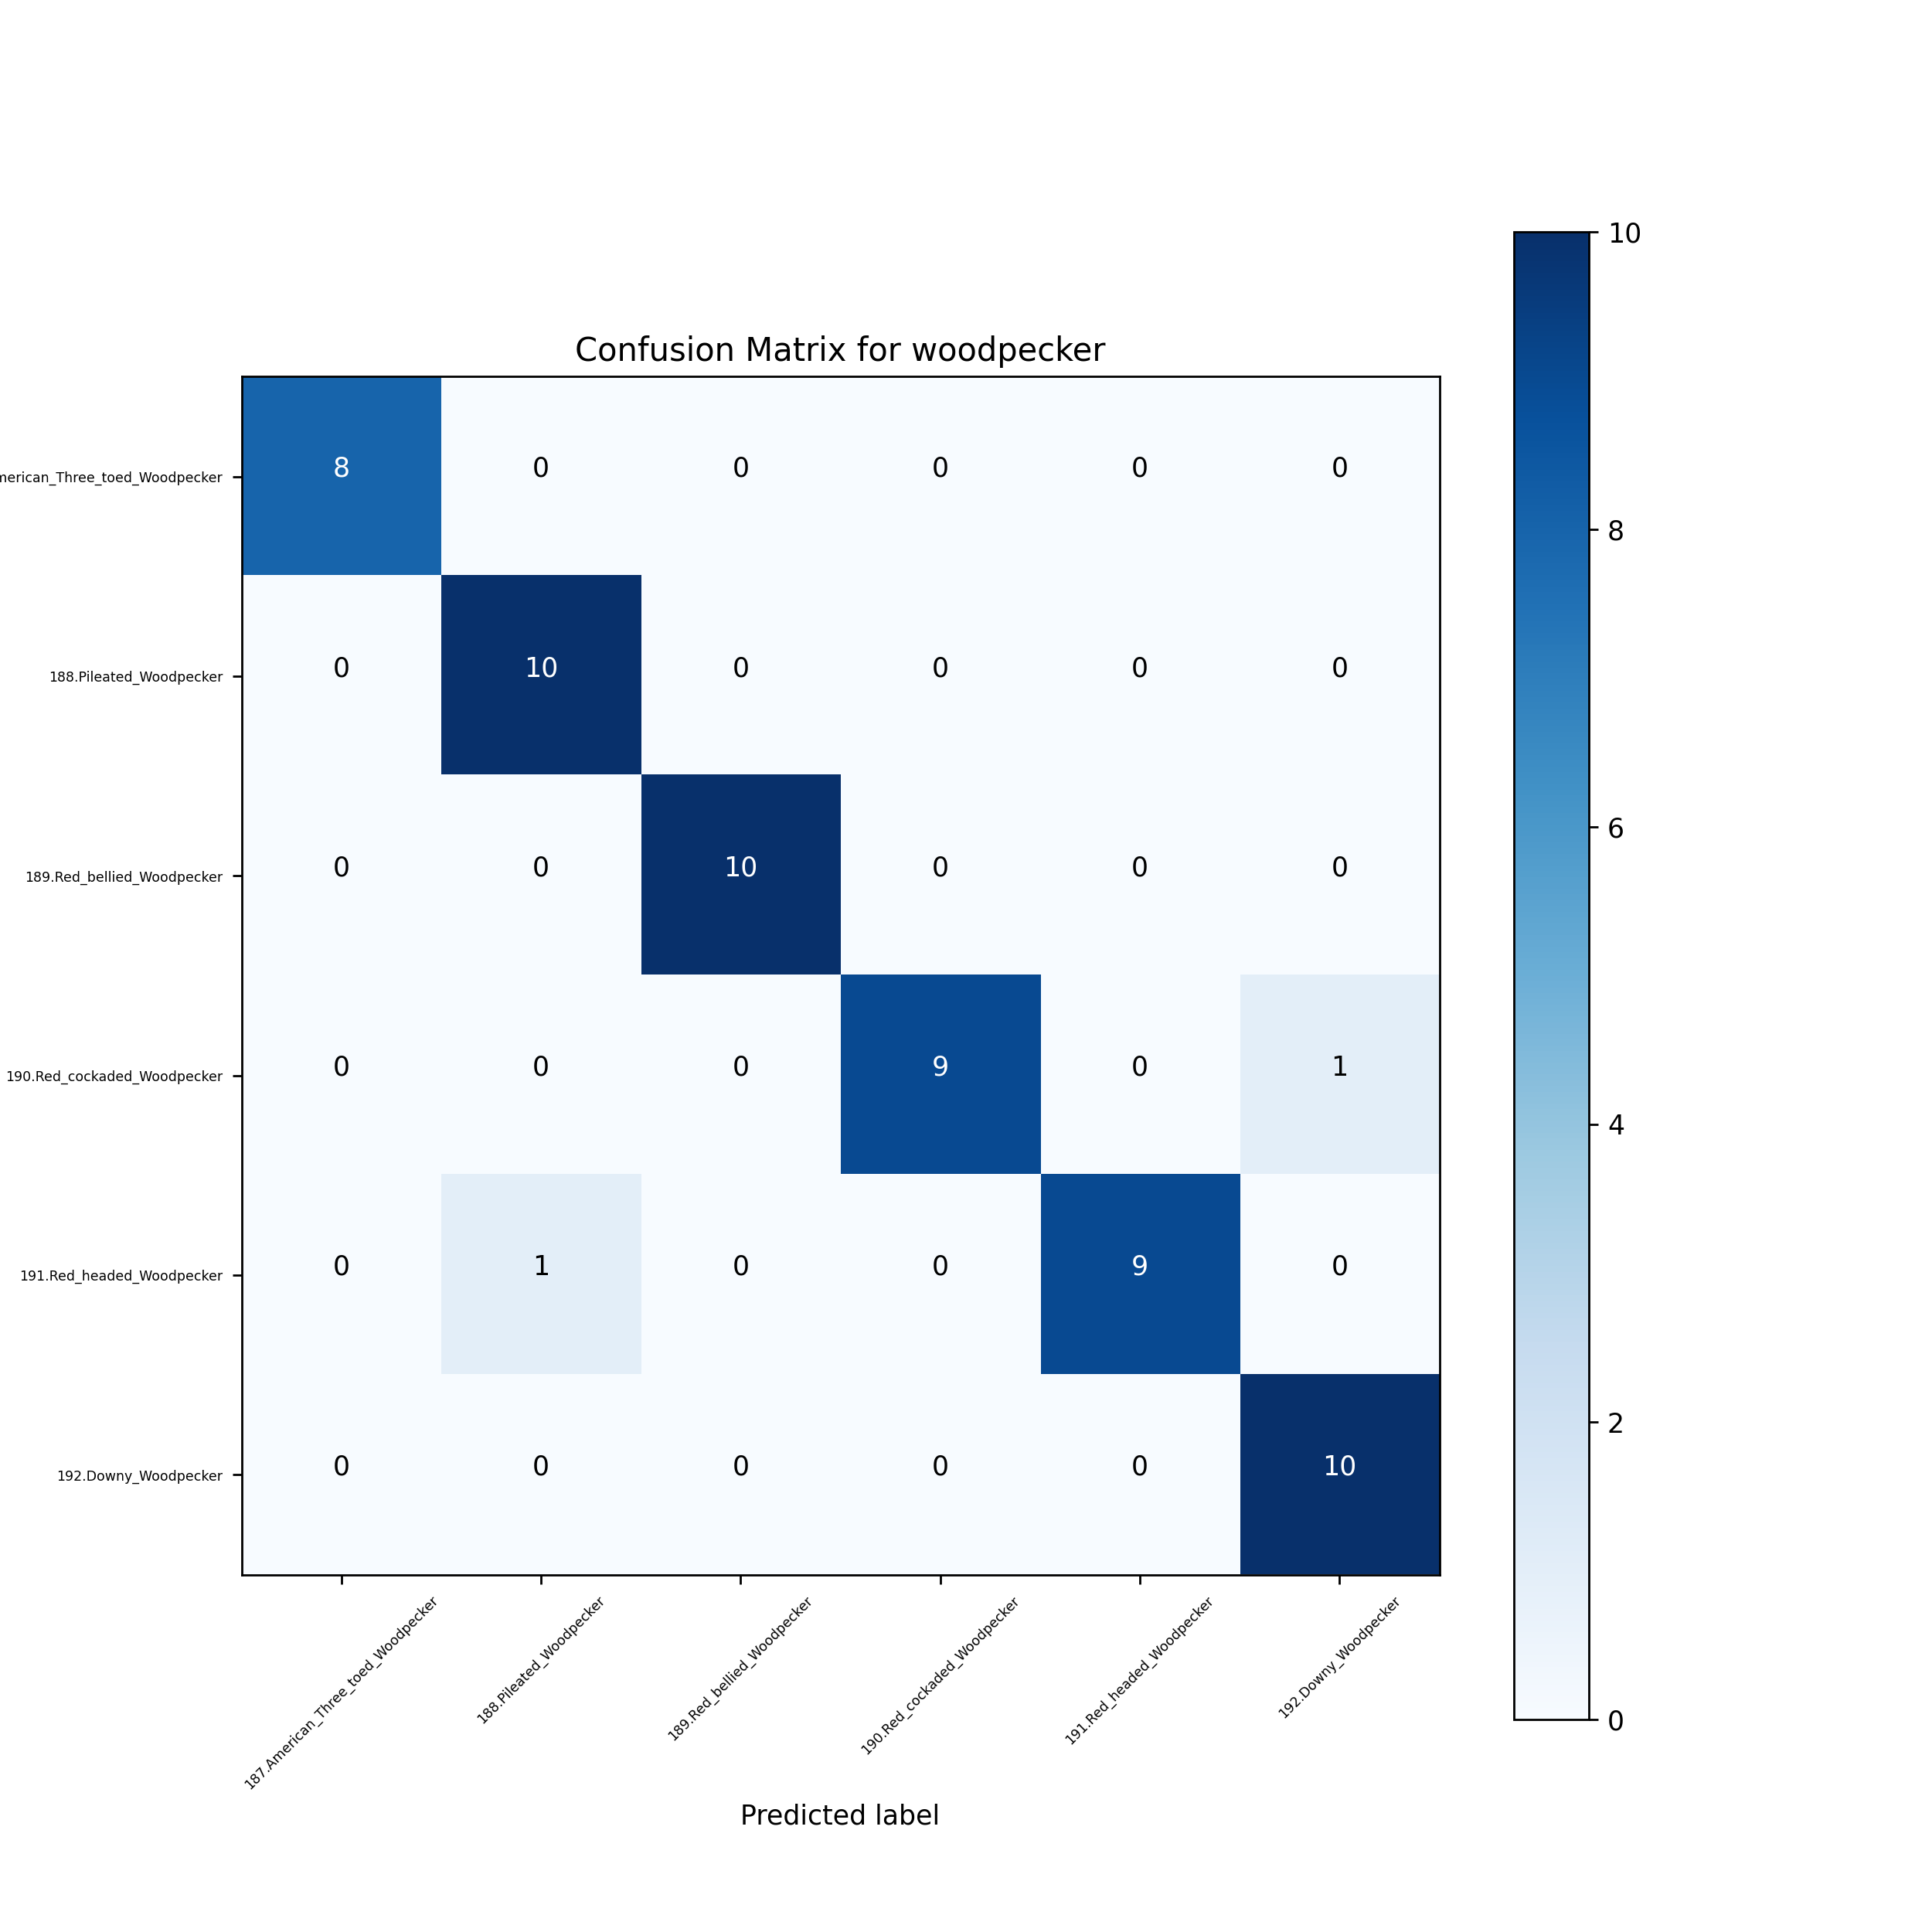
\includegraphics[width=0.95\linewidth]{figure/eval_high_temp_woodpecker}
\caption{The confusion matrix of woodpeckers}
\label{fig:evalhightempwoodpecker}
\end{figure}
\begin{figure}[H]
\centering
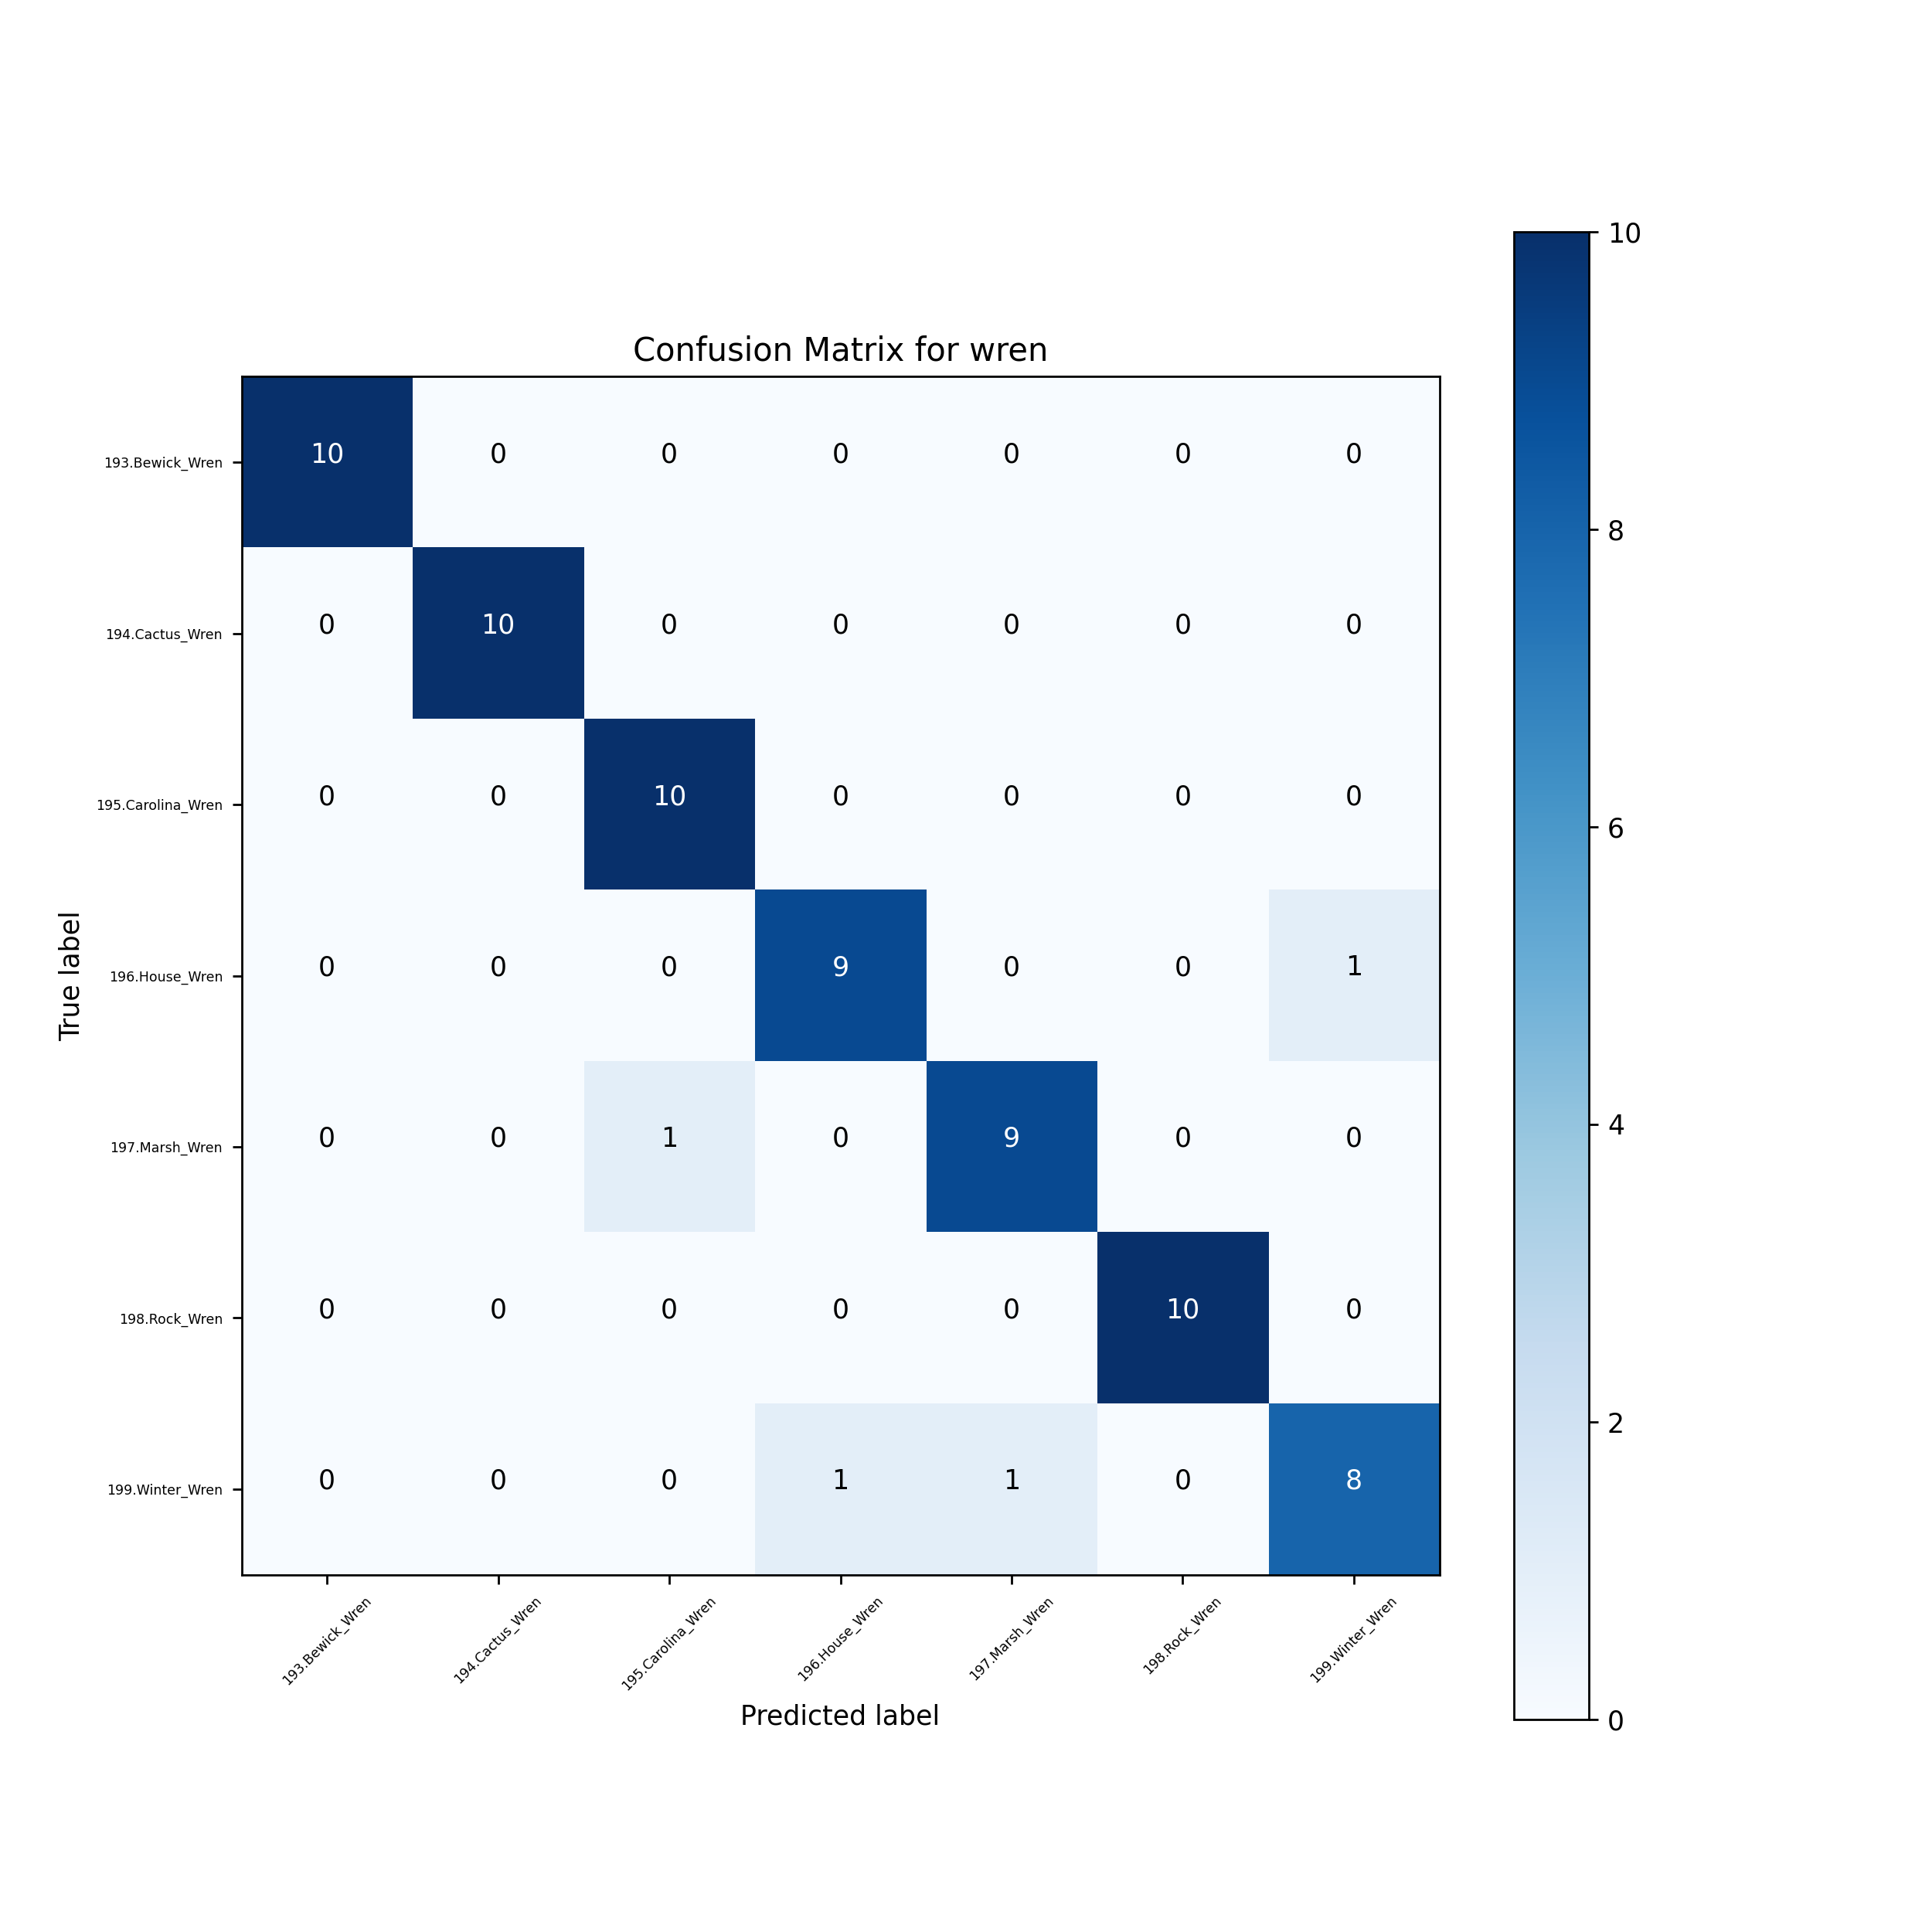
\includegraphics[width=0.95\linewidth]{figure/eval_high_temp_wren}
\caption{The confusion matrix of wrens}
\label{fig:evalhightempwren}
\end{figure}

\subsection{Bugs in HERBS's Official Code}

When running the official code, I found several bugs. For example, in \autoref{fig:combbug}, the author didn't properly pass the \texttt{use\_combiner} parameter into model when building the model. Therefore, if I don't fix this bug, when conducting ablation study, there won't have any difference in model. Another example is \autoref{fig:evalbug}, when importing \texttt{PluginModel}, the original code append ``\texttt{.py}'' to module name.

\begin{figure}[H]
\centering
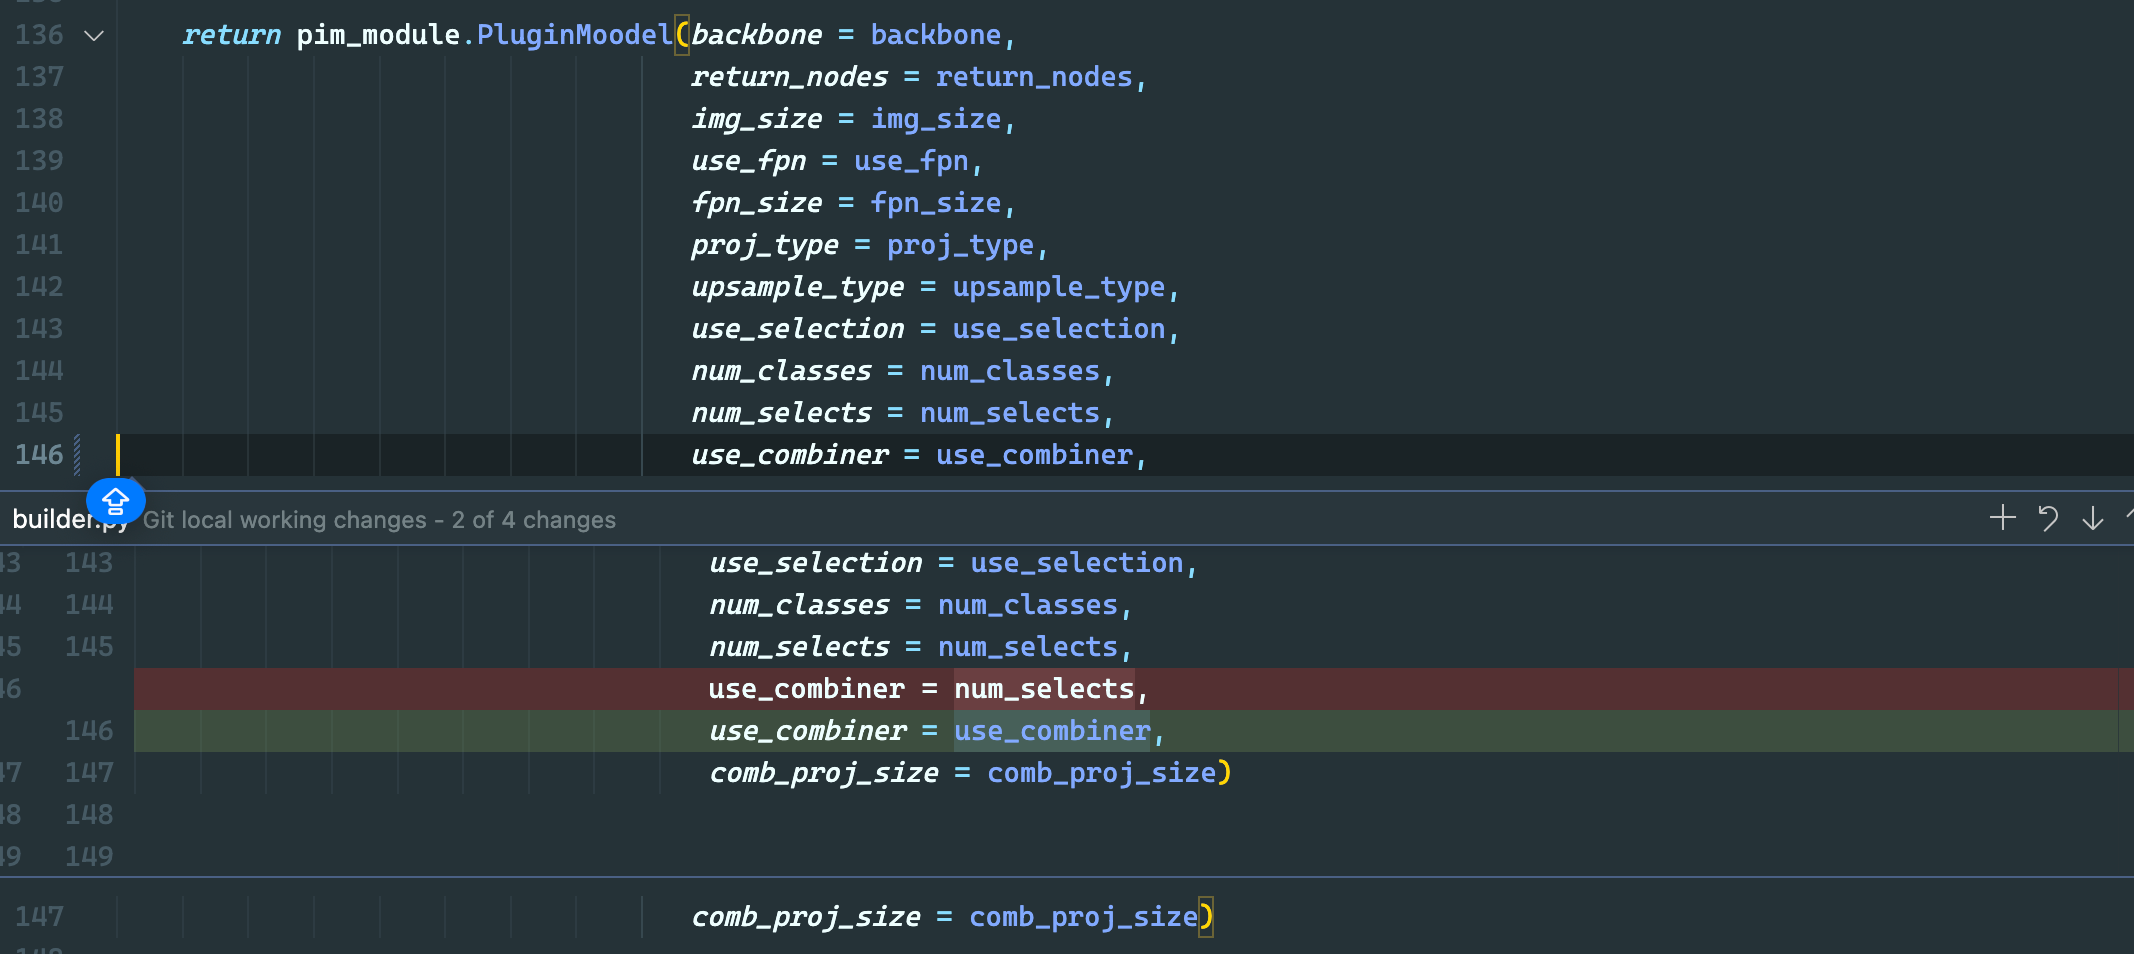
\includegraphics[width=0.95\linewidth]{figure/combbug}
\caption{\texttt{FGVC-HERBS/models/builder.py}. Parameter \texttt{use\_combiner} are not properly passed into model.}
\label{fig:combbug}
\end{figure}

\begin{figure}[H]
\centering
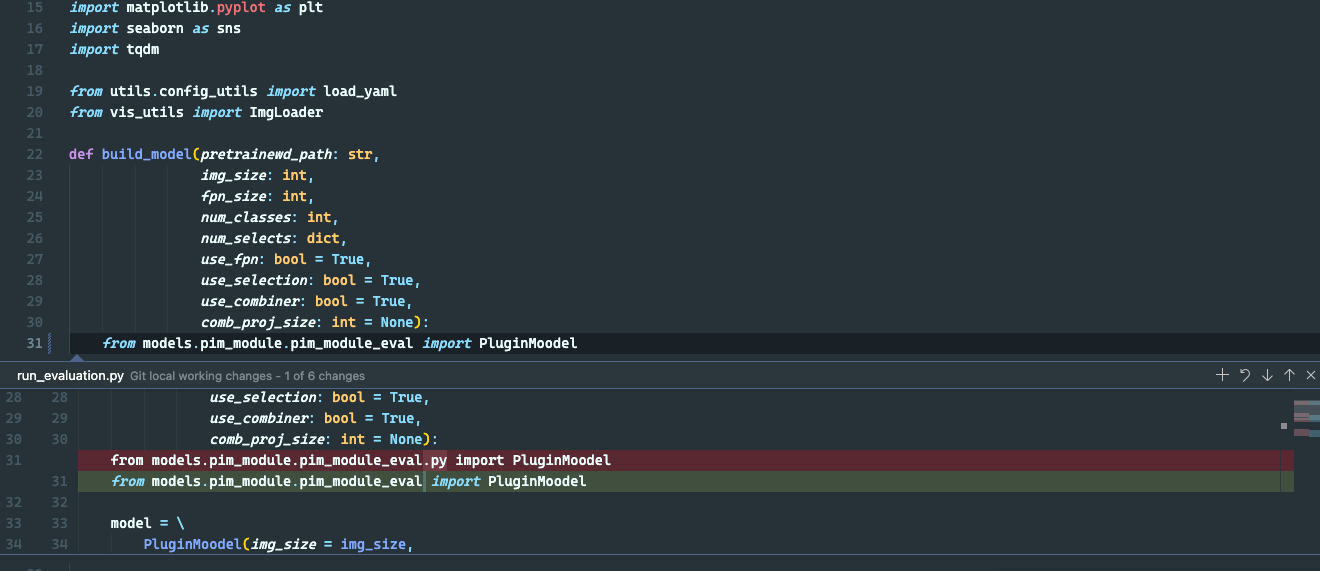
\includegraphics[width=0.95\linewidth]{figure/evalbug}
\caption{\texttt{FGVC-HERBS/run\_evaluation.py}. Error when importing the package.}
\label{fig:evalbug}
\end{figure}



\printbibliography

\end{document}


